\newpage
\chapter{HASIL DAN PEMBAHASAN} \label{Bab IV}

\section{Hasil Penelitian} \label{IV.Hasil}
Pada bagian ini, akan dijelaskan hasil dari setiap tahapan penelitian yang telah dilakukan, mulai dari penyiapan data hingga proses pelatihan model. Pembahasan di dalamnya mencakup bagaimana data akuisisi dataset sinyal, bagaimana data tersebut dibagi menggunakan skema 5-\textit{Fold Cross-Validation}, serta proses pra-pemrosesan data untuk menstandarkan sinyal dari berbagai subjek. Selain itu, sub-bab ini juga menampilkan hasil pelatihan (\textit{training}) model berupa grafik \textit{loss} dari kedua skenario model Mamba (regresi dan klasifikasi). Grafik tersebut digunakan untuk melihat apakah model berhasil belajar dengan baik dan stabil selama proses pelatihan berlangsung.

\subsection{Akuisisi Dataset} \label{IV.Akuisisi}
Dataset yang digunakan dalam penelitian ini merupakan dataset publik bertajuk "The ULg Multimodality Drowsiness Database" (DROZY) yang diperoleh melalui platform terbuka untuk penelitian pemantauan tingkat kantuk \cite{Massoz2016}. Dataset ini mencakup rekaman sinyal fisiologis dari 14 subjek sehat yang menjalani serangkaian sesi eksperimen dalam kondisi kekurangan tidur untuk menginduksi rasa kantuk secara alami. Bahan penelitian yang digunakan terdiri dari 36 set data valid dalam format .edf yang menyertakan label kantuk subjektif serta rekaman \textit{Polysomnography} (PSG). Sinyal fisiologis yang diekstraksi dari dataset ini meliputi 5 kanal EEG (Fz, Cz, Pz, C3, C4) dan 2 kanal EOG (vertikal dan horizontal) dengan frekuensi sampling sebesar 512 Hz. Untuk kebutuhan klasifikasi, label asli dari \textit{Karolinska Sleepiness Scale} (KSS) yang memiliki 9 tingkatan dikategorikan ulang menjadi dua kelas utama, yaitu Alert (KSS 1-5) dan Drowsy (KSS 6-9). Visualisasi perbandingan contoh sinyal mentah dari ketujuh kanal untuk setiap kategori tingkat kantuk tersebut disajikan pada Gambar \ref{fig:class-sign}.

\begin{figure}[H]
    \centering
    % --- Gambar Kiri ---
    \begin{subfigure}[b]{0.48\textwidth} % Pakai 0.48 biar ada gap dikit di tengah
        \centering
        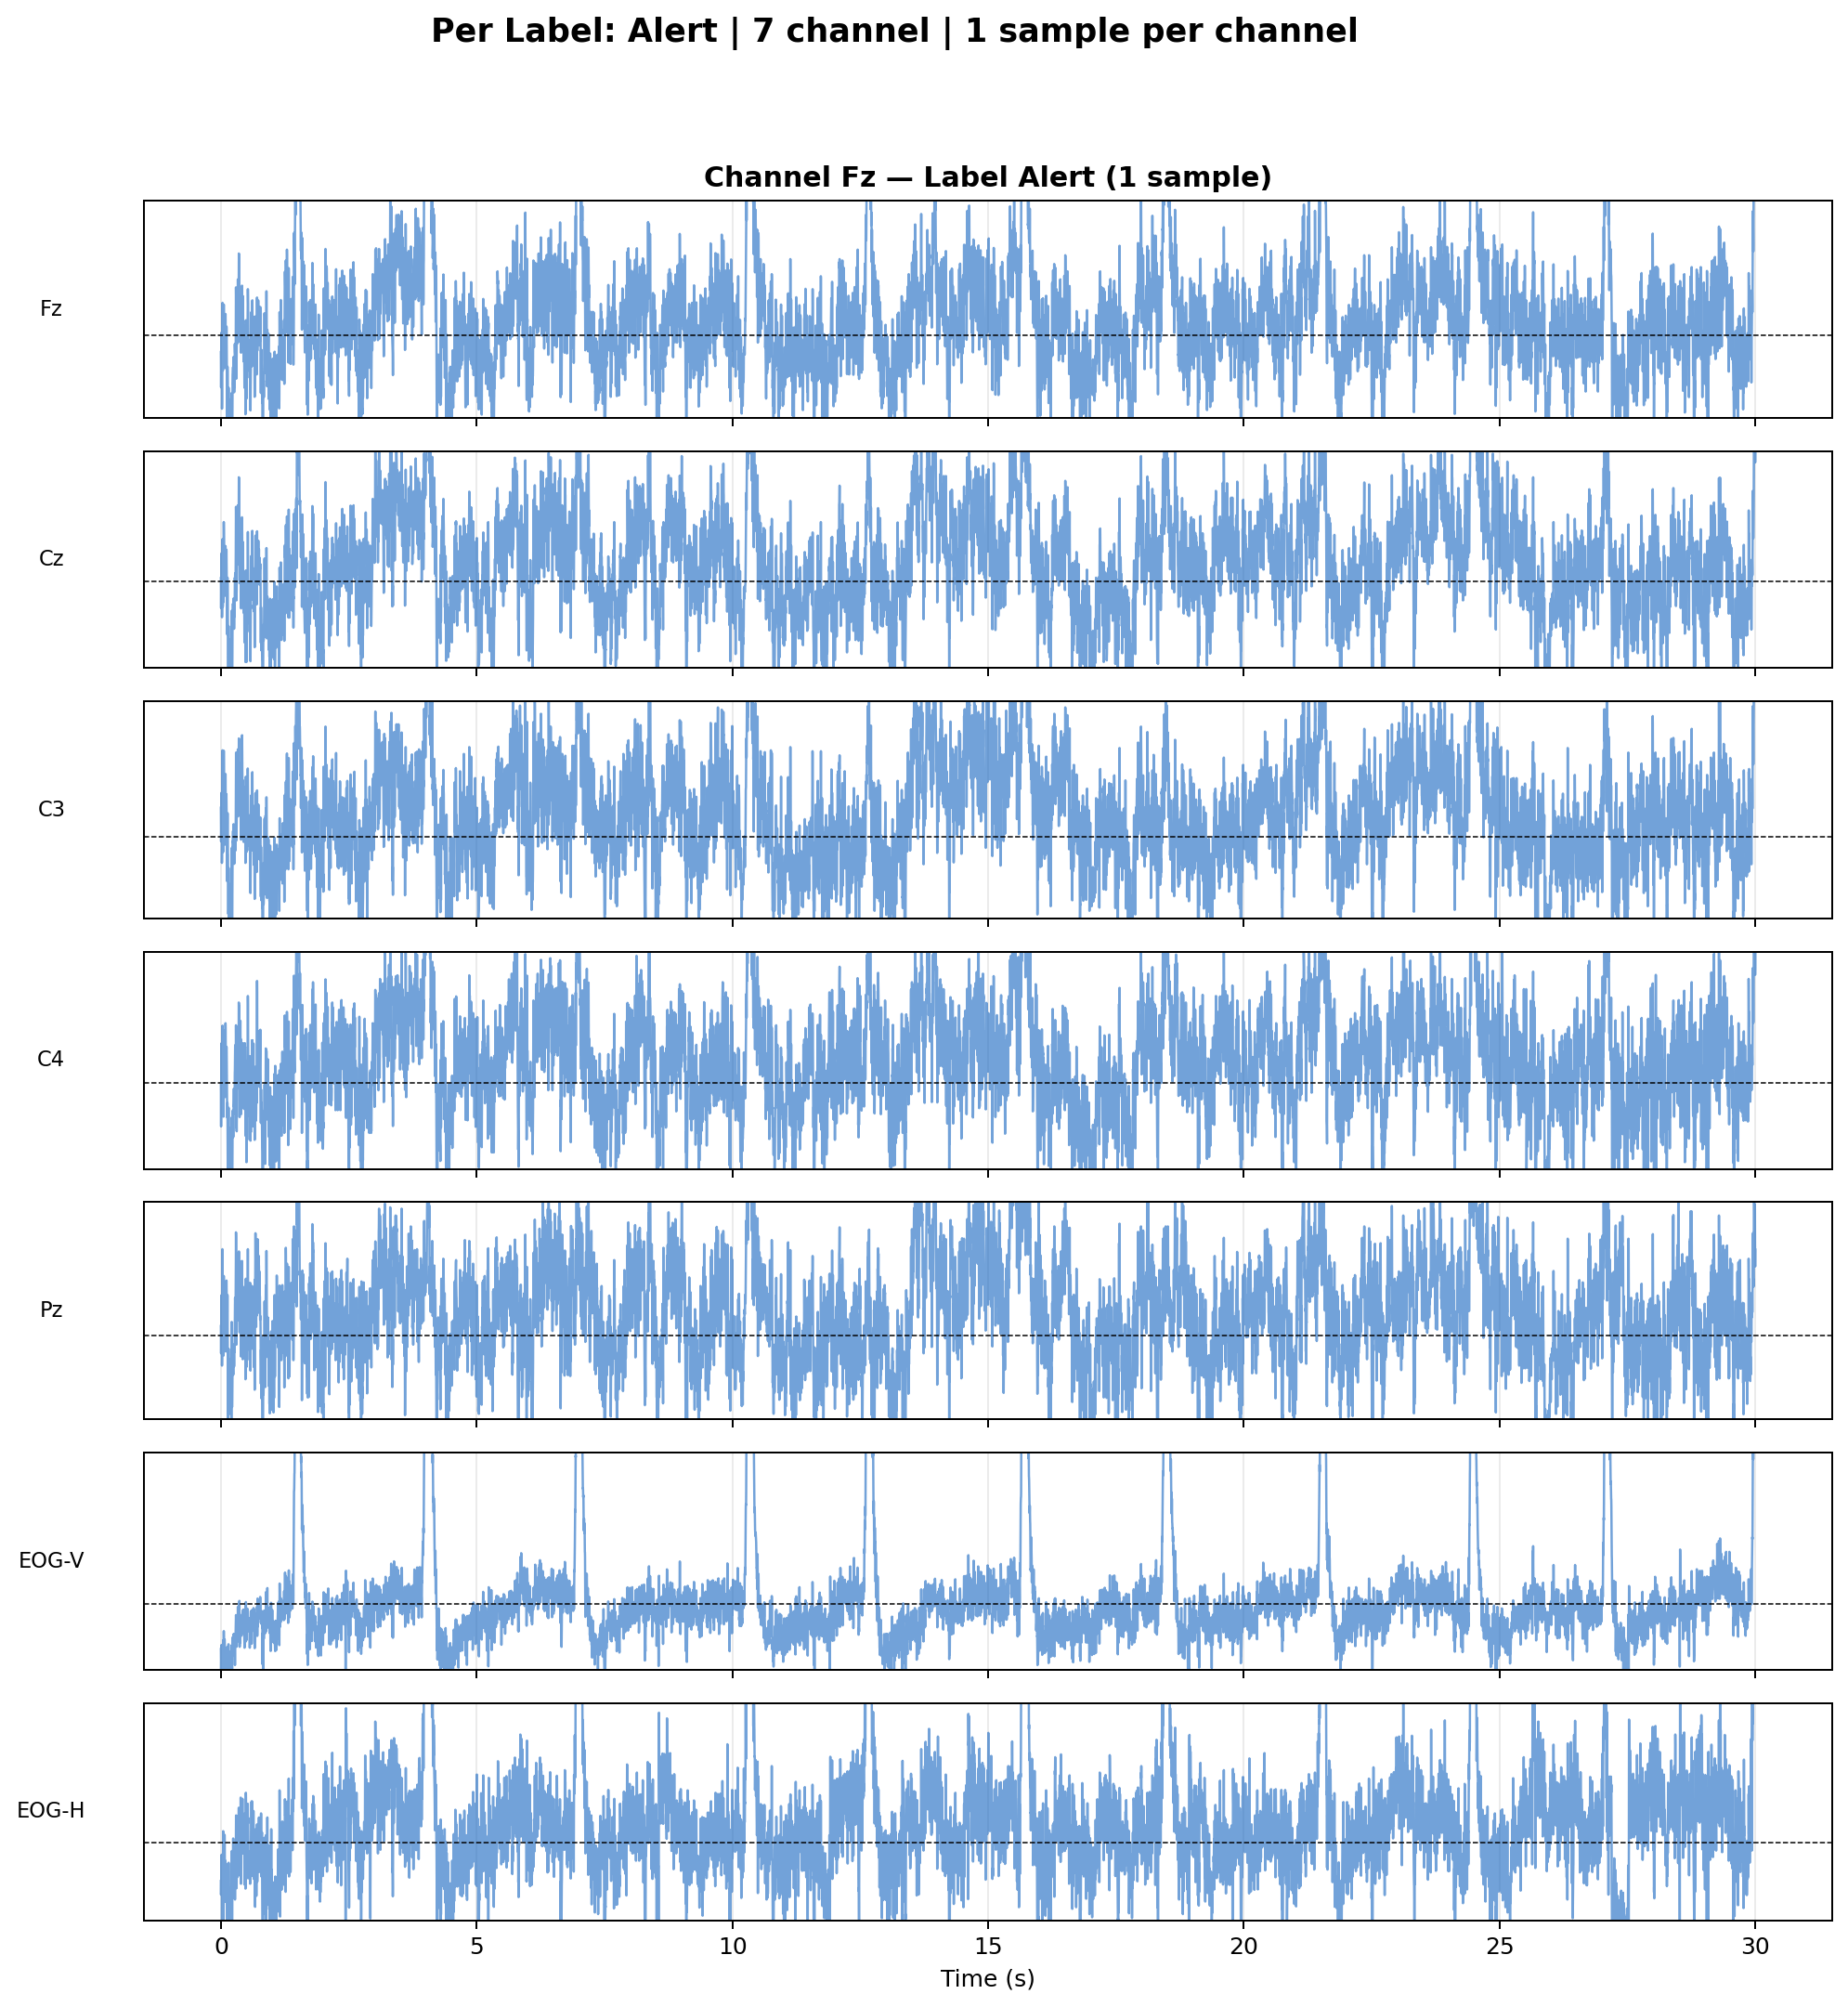
\includegraphics[width=\linewidth]{figure/label_Alert_channel_traces.png}
        \caption{Sinyal \textit{Alert}}
        \label{fig:alert-sign}
    \end{subfigure}
    \hfill % Ini buat dorong gambar ke ujung kiri dan kanan (kasih gap otomatis)
    % --- Gambar Kanan ---
    \begin{subfigure}[b]{0.48\textwidth}
        \centering
        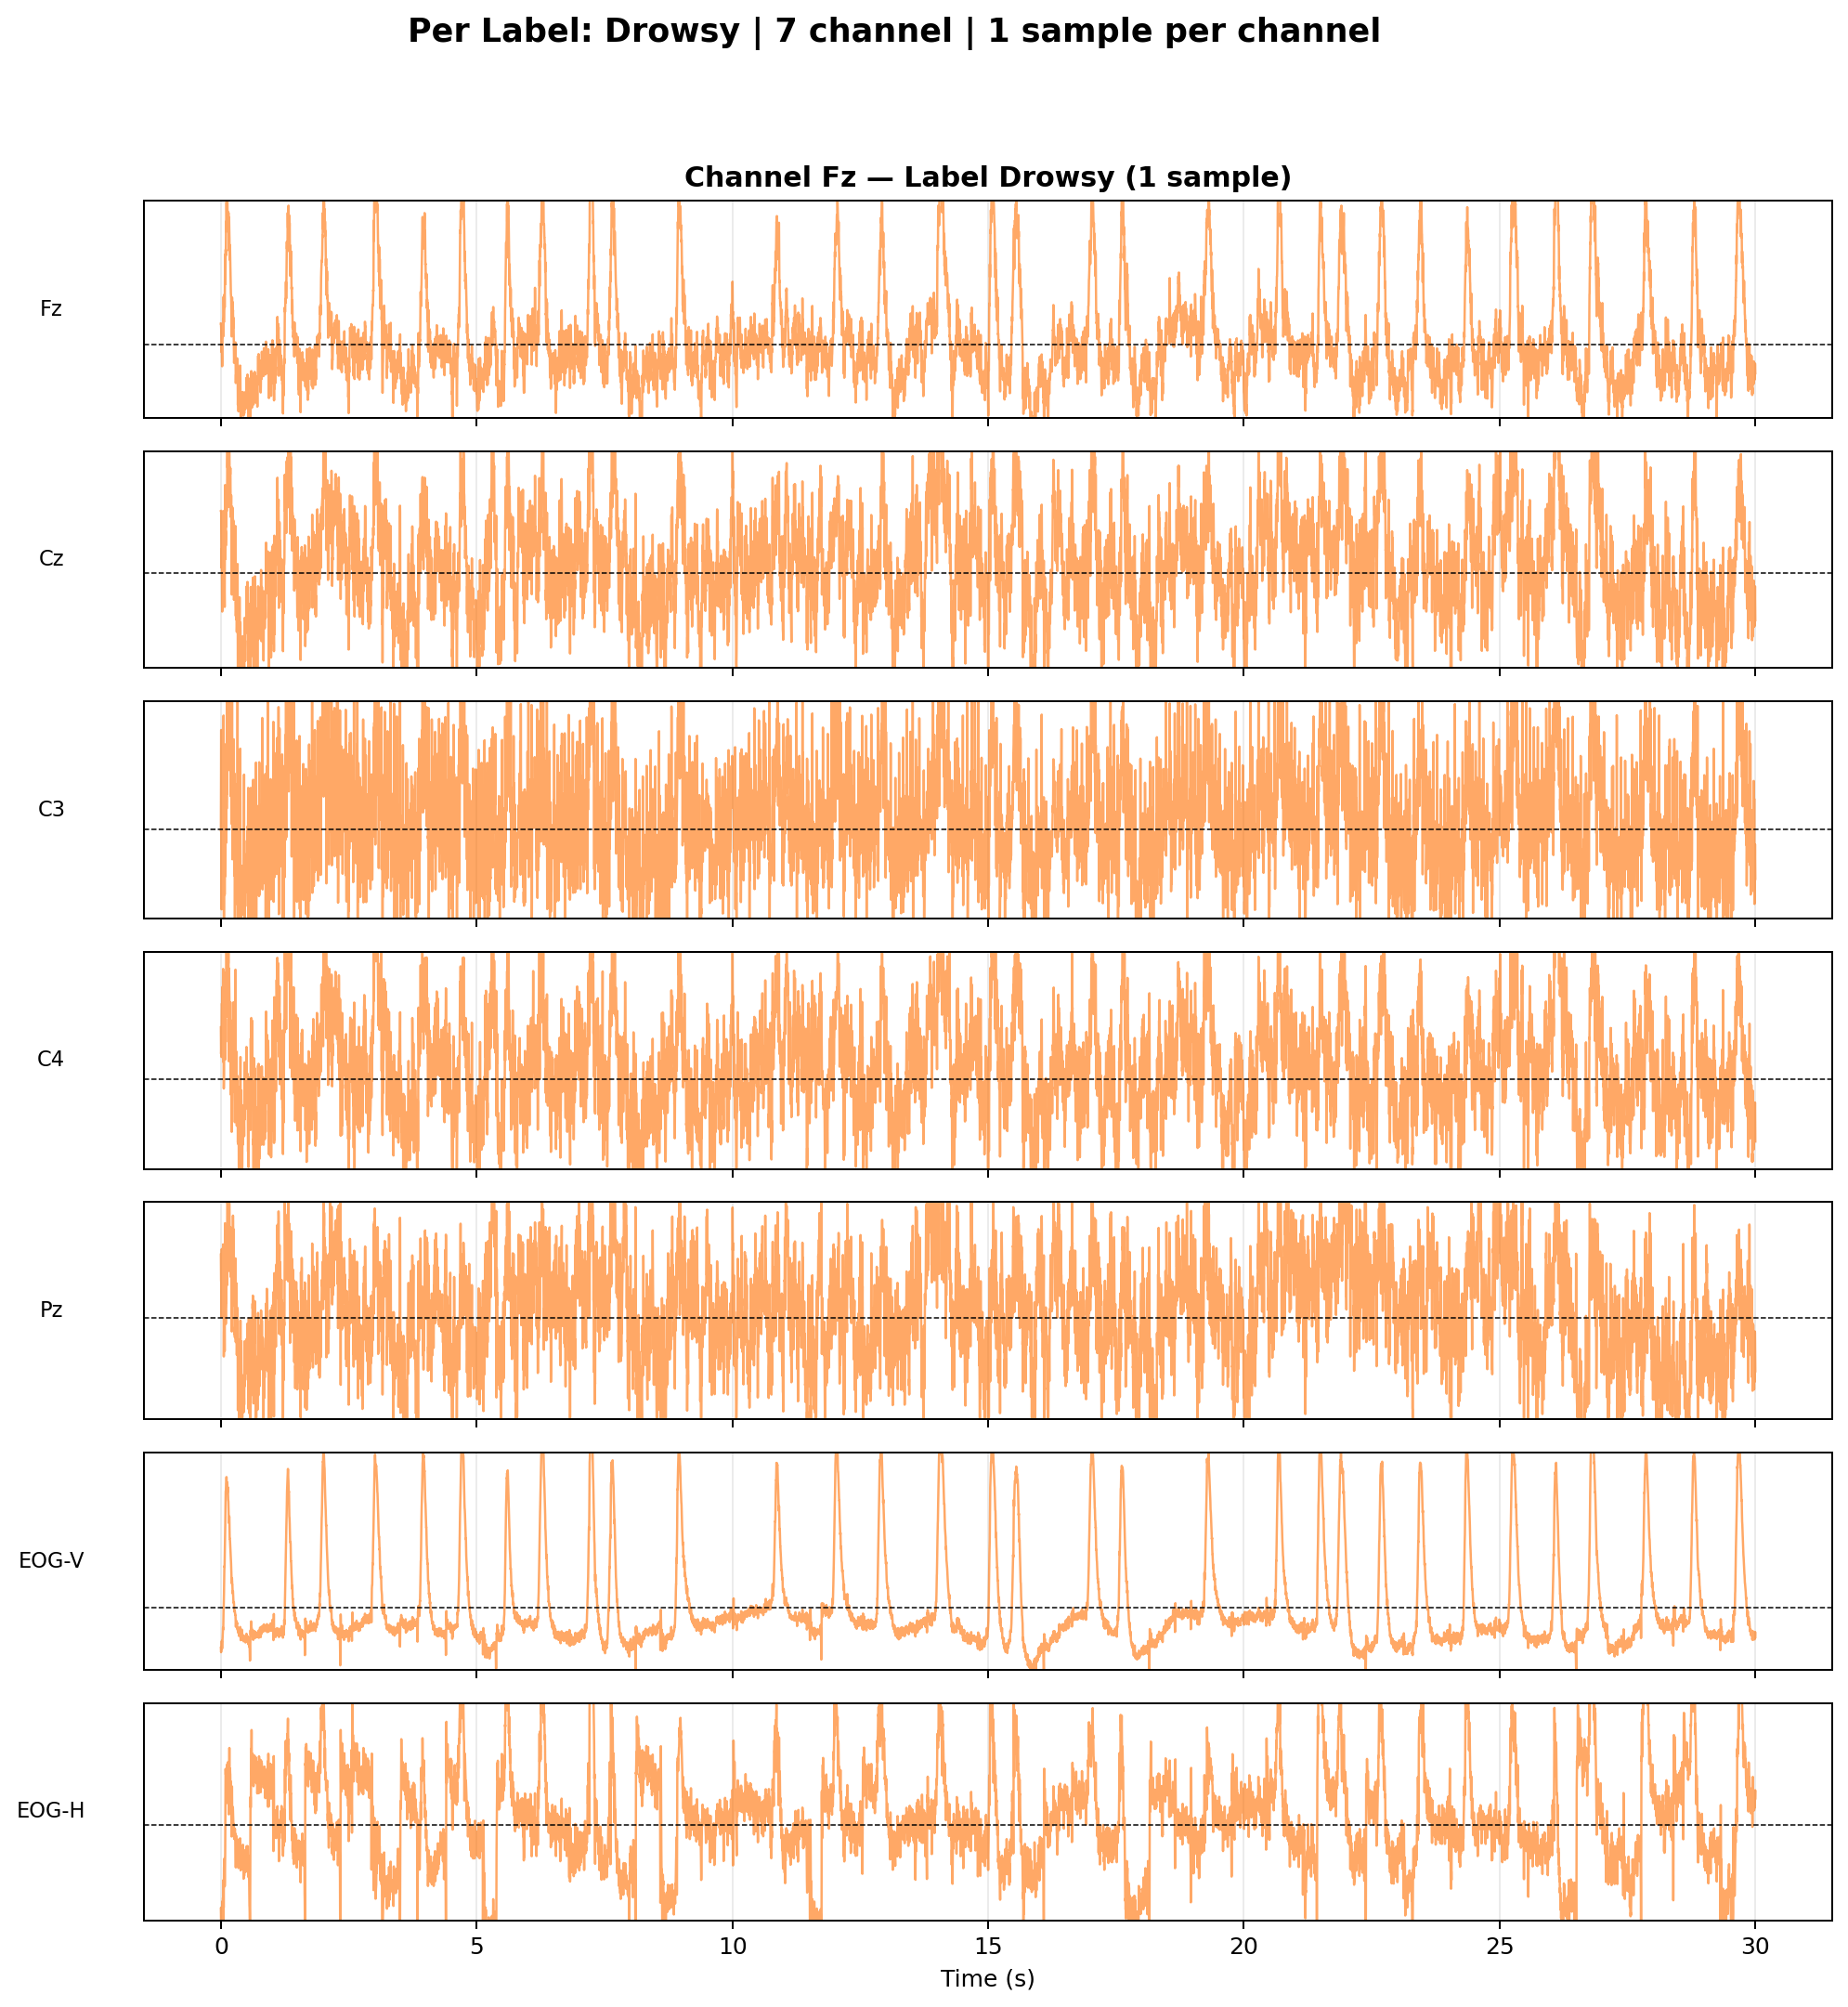
\includegraphics[width=\linewidth]{figure/label_Drowsy_channel_traces.png}
        \caption{Sinyal \textit{Drowsy}}
        \label{fig:drowsy-sign}
    \end{subfigure}

    \caption{Contoh Sinyal dari Kedua Kelas Tingkat Kantuk}
    \label{fig:class-sign}
\end{figure}

\subsection{Pembagian Dataset}
Dataset yang telah disegmentasi dibagi menjadi lima bagian (fold) menggunakan skema Subject-Wise K-Fold Cross Validation dengan nilai $k=5$. Melalui pendekatan ini, seluruh rekaman yang berasal dari satu subjek ditempatkan secara eksklusif pada satu fold yang sama untuk menjaga kemandirian data uji terhadap karakteristik individu. Total rekaman yang digunakan adalah 36 sesi dari 14 subjek yang menghasilkan sejumlah segmen berdurasi 30 detik. Detail pembagian subjek dan persebaran jumlah sampel untuk setiap kelas pada masing-masing fold disajikan dalam Tabel \ref{tab:sebaran_fold} . \par

\begin{table}[H]
    \centering
    \caption{Skema Pembagian Subjek pada 5-Fold Cross-Validation}
    \label{tab:sebaran_fold}
    \begin{tabular}{|c|p{4cm}|c|}
        \hline
        \textbf{Fold ke-} & \textbf{Data Latih (Subjek)} & \textbf{Data Validasi (Subjek)} \\ \hline
        1 & 1, 10, 11, 13, 14, 2, 3, 5, 6, 7, 8 & 12, 4, 9 \\ \hline
        2 & 1, 10, 12, 13, 14, 2, 4, 5, 6, 7, 9 & 11, 13, 8 \\ \hline
        3 & 1, 11, 12, 13, 14, 3, 4, 5, 6, 8, 9 & 10, 2, 7 \\ \hline
        4 & 10, 11, 12, 13, 2, 3, 4, 5, 7, 8, 9 & 1, 14, 6 \\ \hline
        5 & 1, 10, 11, 12, 14, 2, 3, 4, 6, 7, 8, 9 & 13, 5 \\ \hline
    \end{tabular}
\end{table}

\subsection{Prapemrosesan Data}
Pada tahap ini, dataset melalui proses prapemrosesan sebelum dimasukkan ke dalam model untuk tahapan pelatihan. Tahapan ini sangat krusial guna mengubah data sinyal PSG mentah menjadi format sekuensial terstruktur yang siap diolah oleh arsitektur Mamba. Langkah pertama yang dilakukan adalah segmentasi sinyal menggunakan teknik \textit{sliding window}. Sinyal kontinu dari 7 kanal (5 kanal EEG dan 2 kanal EOG) dipotong menjadi segmen-segmen dengan \textit{window size} selama 30 detik. Pemotongan ini diatur menggunakan parameter pergeseran (\textit{stride}) sebesar 10 detik, yang secara otomatis menghasilkan area \textit{overlap} antar-segmen yang berdekatan sebesar 20 detik. Berdasarkan frekuensi \textit{sampling} bawaan sebesar 512 Hz, setiap segmen 30 detik tersebut akan diekstrak menjadi matriks atau tensor berukuran $[7 \times 15.360]$ titik data, yang kemudian diperlakukan sebagai satu sampel data individual. Pendekatan \textit{overlap} ini sangat efektif untuk melipatgandakan jumlah sampel data sekaligus mempertahankan kontinuitas konteks temporal perubahan fase kantuk dari waktu ke waktu. Detail implementasi algoritma \textit{sliding window} pada proses segmentasi dataset ini direpresentasikan pada Kode \ref{code:windowing}. 

\begin{lstlisting}[language=Python, caption=Kode Segmentasi Data, label={code:windowing}]
# config.py
WINDOW_SEC = 30
STRIDE_SEC = 10

# train.py
window_sec=Config.WINDOW_SEC
stride_sec=Config.STRIDE_SEC

try:
    raw_info     = mne.io.read_raw_edf(file_path, preload=False, verbose='error')
    duration_sec = raw_info.times[-1]

    max_start = duration_sec - self.window_sec

    if max_start <= 0:
        print(f"  [SKIP] {filename}: terlalu pendek ({duration_sec:.1f}s)")
        continue

    subject_id = filename.split('-')[0]
    for start in np.arange(0, max_start, self.stride_sec):
        self.samples.append({
            'file_path':  file_path,
            'start_sec':  float(start),
            'label':      label,         
            'class_idx':  kss_to_class(label),
            'subject_id': subject_id
        })
        total_windows += 1

except Exception as e:
    print(f"  [ERROR] {filename}: {e}")
\end{lstlisting}

Langkah kedua adalah penerapan Normalisasi Z-Score atau standardisasi untuk menyeragamkan skala setiap fitur sinyal. Dalam penelitian ini, normalisasi dilakukan secara spesifik per subjek untuk mengeliminasi perbedaan karakteristik neurofisiologis antar individu yang dapat memengaruhi objektivitas model. Dengan menyamakan distribusi data melalui nilai rata-rata (mean) dan standar deviasi, metode ini berfungsi untuk memitigasi masalah pergeseran domain antara data pelatihan dan data pengujian. Untuk menjaga validitas evaluasi dan mencegah kebocoran data, parameter statistik ($\mu$ dan $\sigma$) dihitung hanya berdasarkan data latih pada setiap fold dalam skema subject-wise K-Fold Cross Validation, yang kemudian diaplikasikan secara konsisten pada data uji di fold yang bersesuaian. Implementasi kode prapemrosesan ini disajikan pada Kode~\ref{code:preprocessing}. \par

\begin{lstlisting}[language=Python, caption=Kode Normalisasi, label={code:preprocessing}]
norm_mode = getattr(Config, 'NORMALIZATION', 'window')
if norm_mode == 'subject' and hasattr(self, 'subject_stats'):
	subject_id = info.get('subject_id', os.path.basename(file_path).split('-')[0])
	subject_stats = self.subject_stats.get(subject_id)
	if subject_stats is not None:
		mean, std = subject_stats
		signal = (signal - mean) / (std + 1e-6)
	else:
		mean = np.mean(signal, axis=1, keepdims=True)
		std = np.std(signal, axis=1, keepdims=True)
		signal = (signal - mean) / (std + 1e-6)
\end{lstlisting}

Gambar \ref{fig:4.norm} menyajikan representasi visual dari hasil penerapan normalisasi sinyal per subjek. Grafik pada sisi kiri menampilkan kondisi sinyal mentah sebelum dinormalisasi, yang masih memiliki rentang skala amplitudo yang sangat lebar. Sebaliknya, grafik pada sisi kanan menunjukkan sinyal setelah dinormalisasi, di mana rentang nilai amplitudonya telah menyusut secara signifikan dan berskala jauh lebih seragam.

\begin{figure}[H]
    \centering
    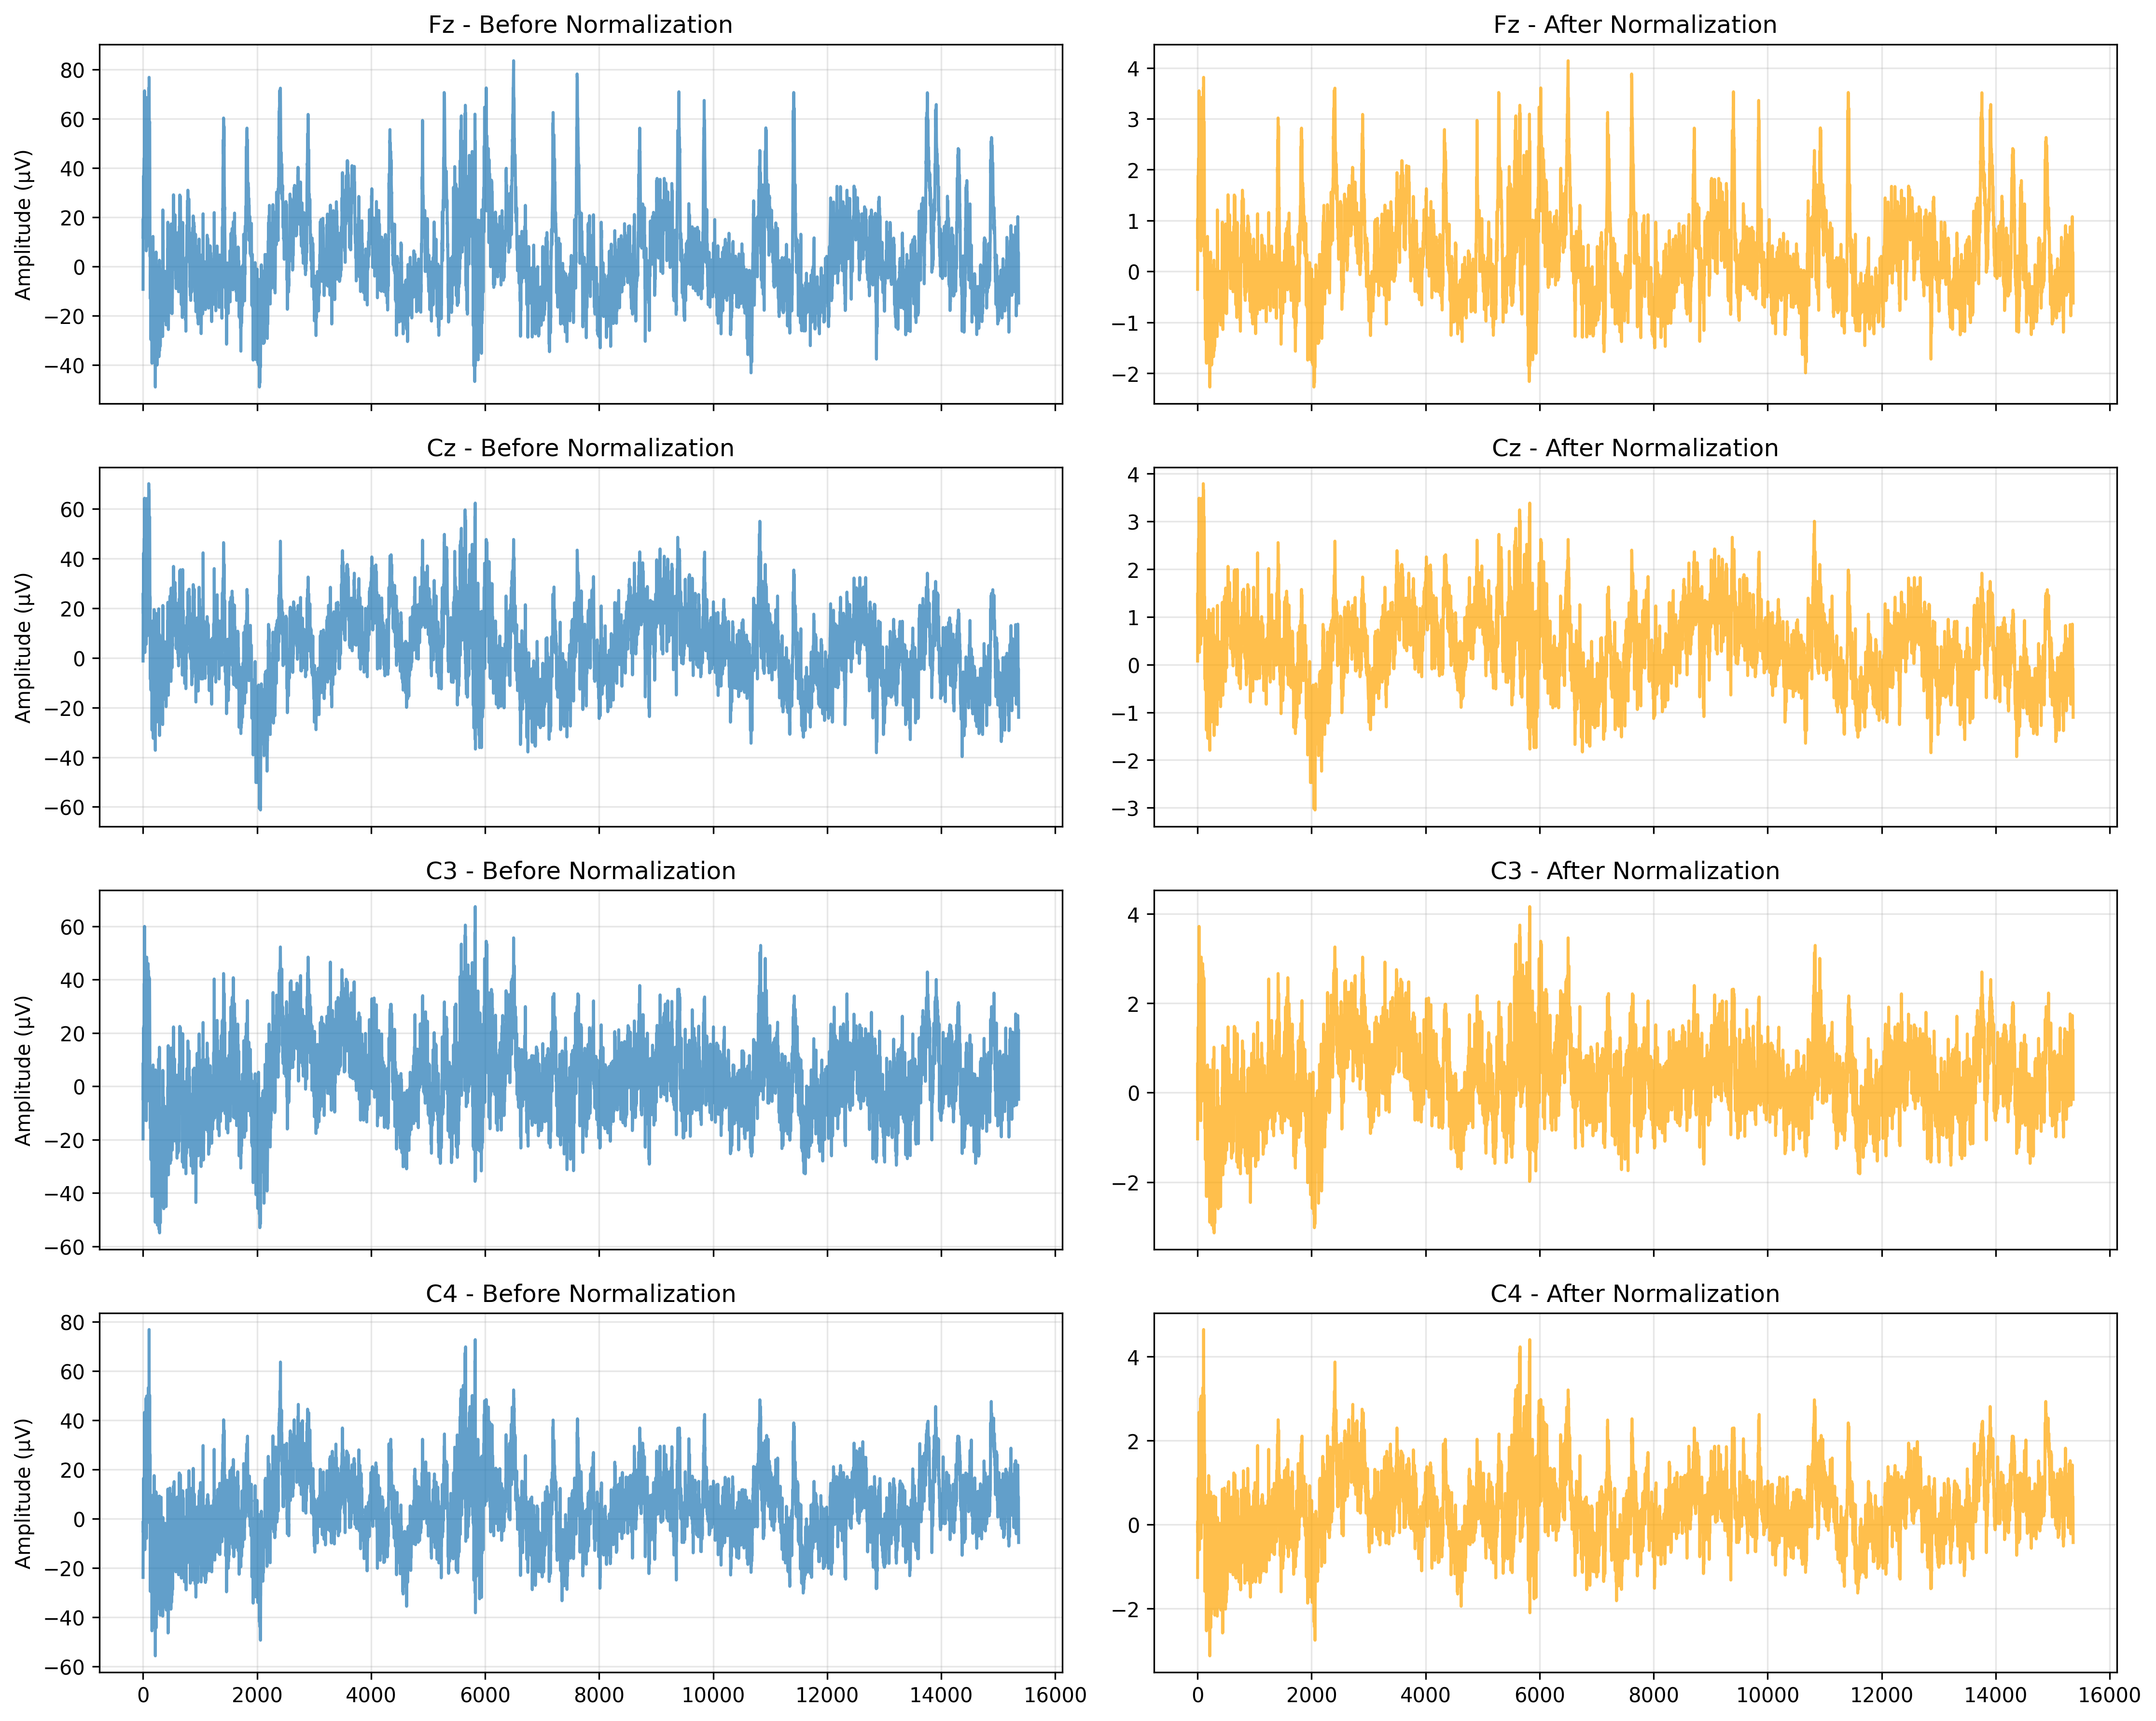
\includegraphics[width=1\textwidth]{figure/signal_normalization_comparison.png}
    \caption{Perbandingan Sinyal Sebelum \& Sesudah Normalisasi}
    \label{fig:4.norm}
\end{figure}

\subsection{Augmentasi Data}
\label{subsec:hasil_augmentasi}

\begin{figure}[H]
    \centering
    % Gambar Pertama (Atas)
    \begin{subfigure}[b]{0.8\textwidth} % Lebar digedein biar enak dilihat
        \centering
        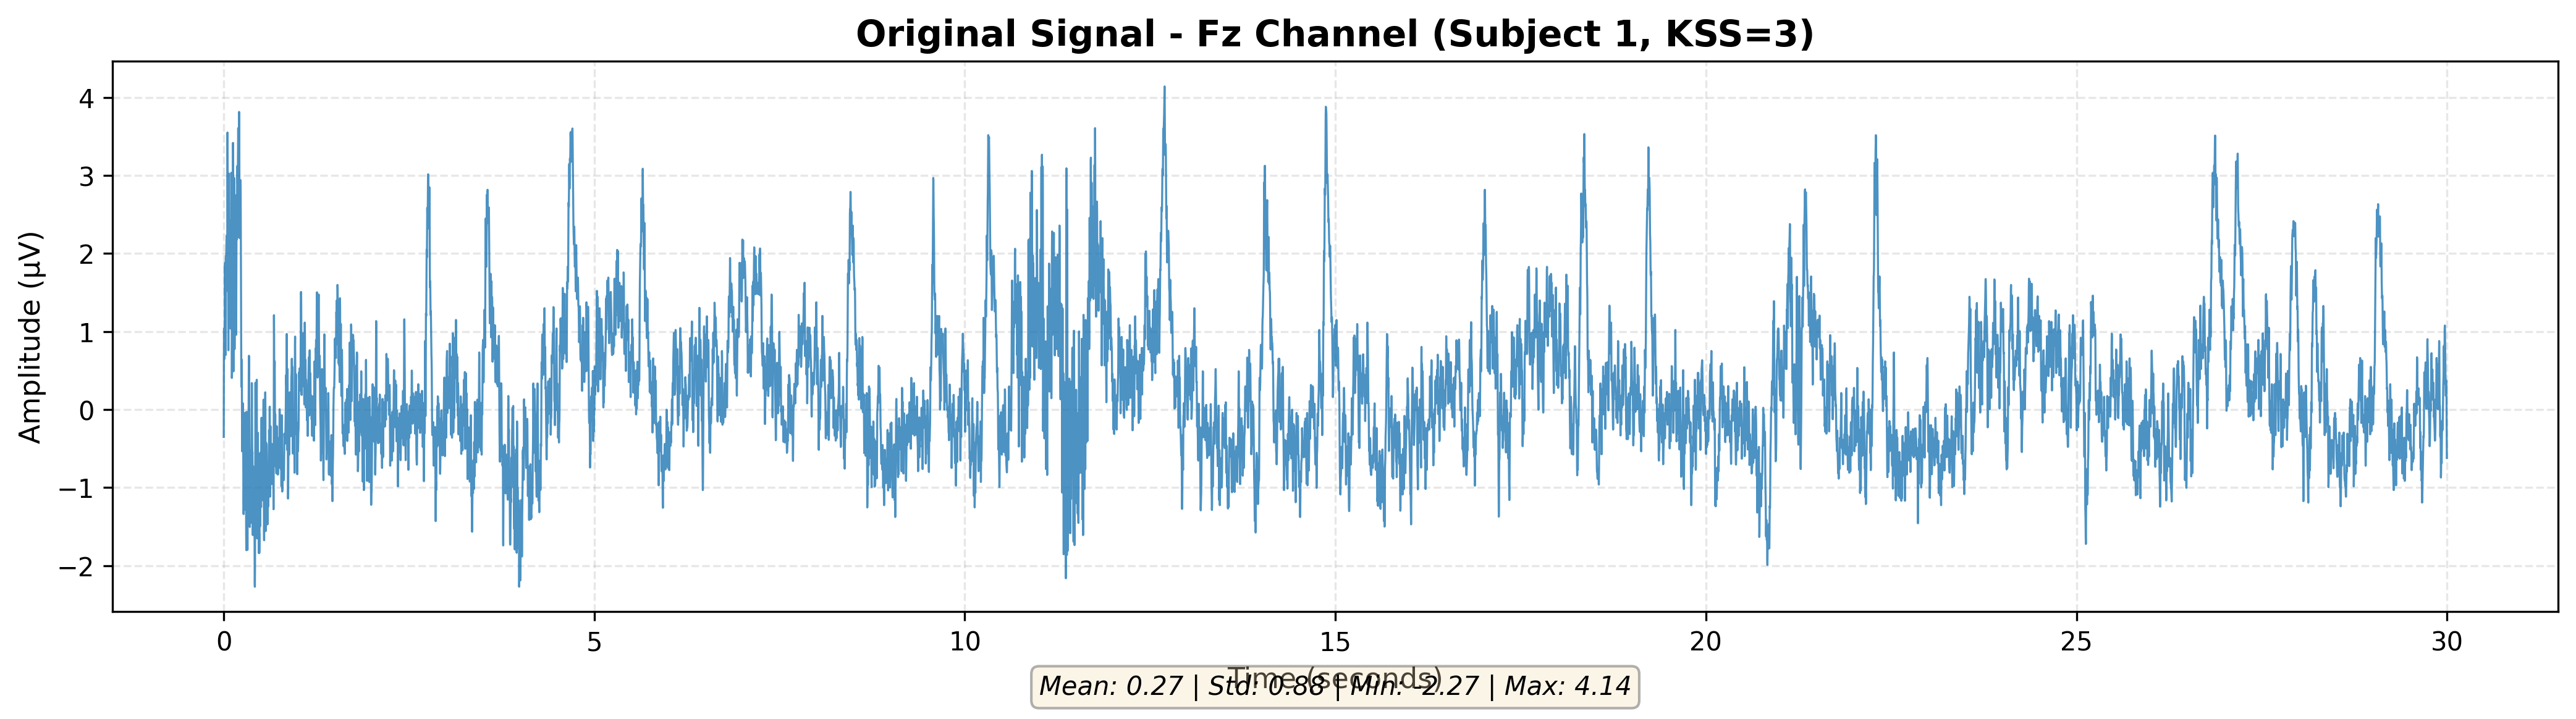
\includegraphics[width=\linewidth]{figure/01_original_signal.png}
        \caption{Sinyal Original}
        \label{fig:ori_sign}
    \end{subfigure}
    
    \vspace{1em}

    % Gambar Kedua (Tengah)
    \begin{subfigure}[b]{0.8\textwidth}
        \centering
        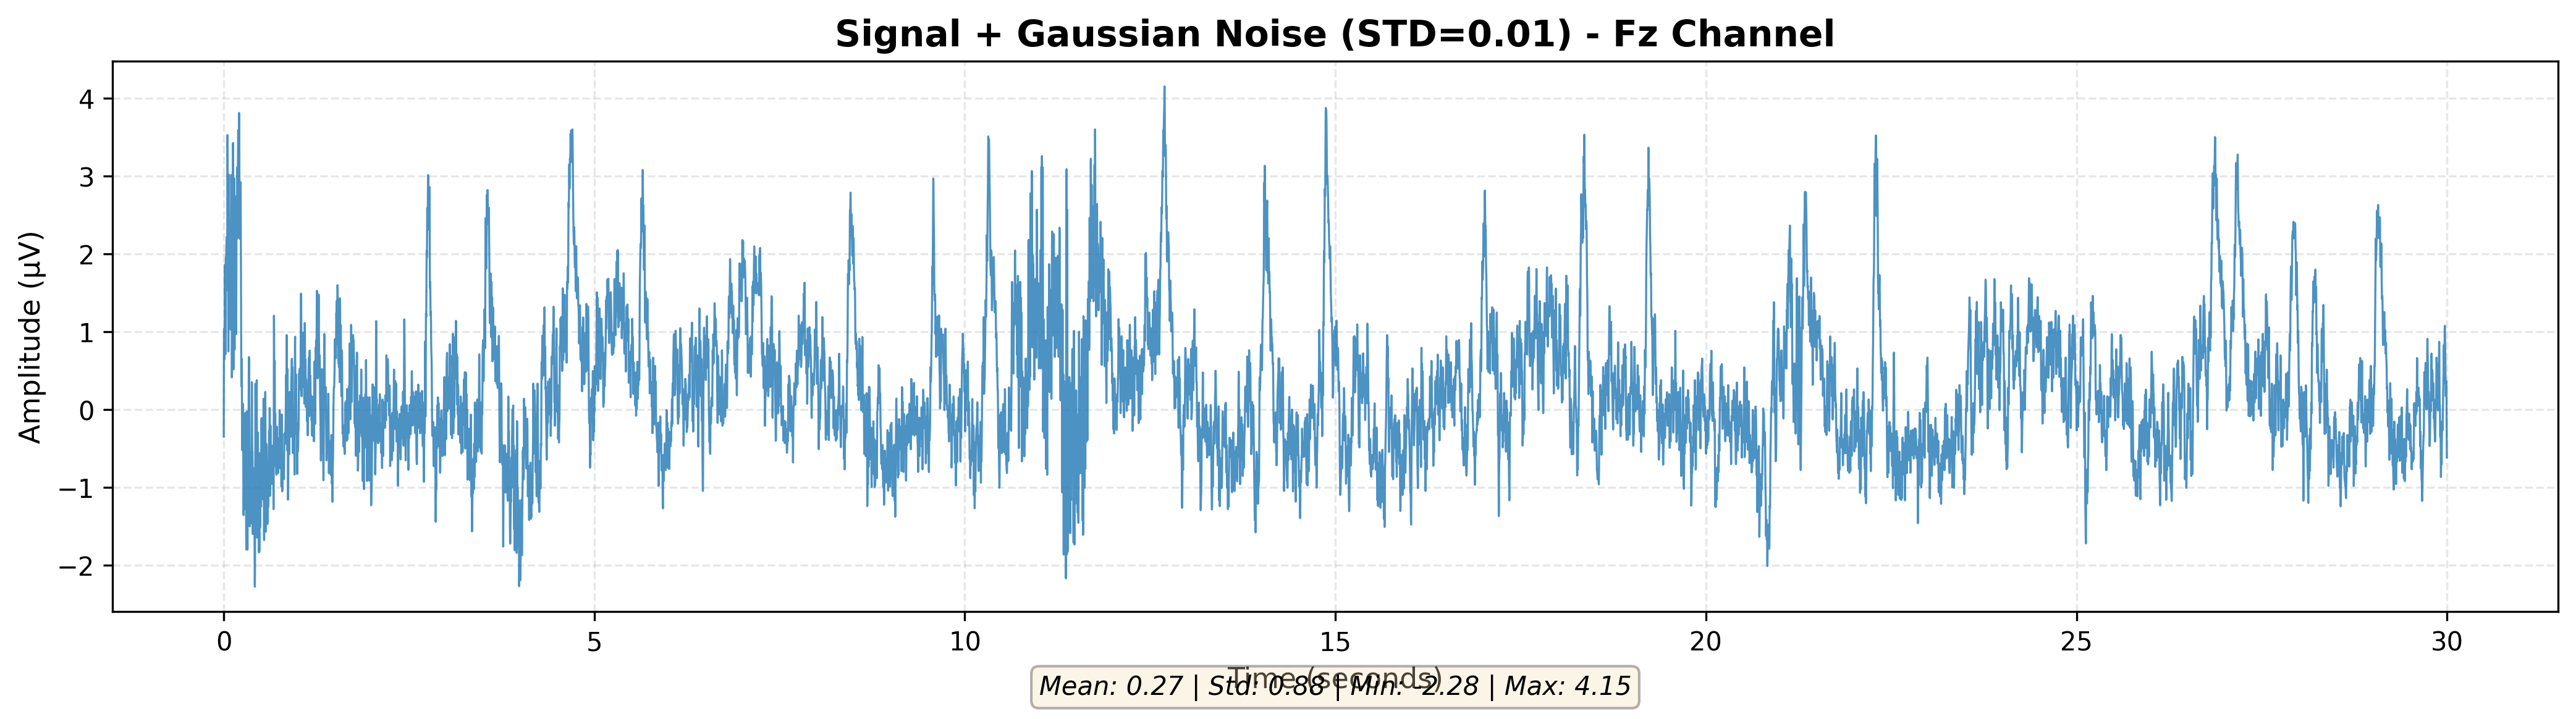
\includegraphics[width=\linewidth]{figure/02_gaussian_noise.png}
        \caption{Sinyal dengan Gaussian Noise}
        \label{fig:gauss_sign}
    \end{subfigure}

    \vspace{1em} % Kasih jarak lagi, anjay

    % Gambar Ketiga (Bawah)
    \begin{subfigure}[b]{0.8\textwidth}
        \centering
        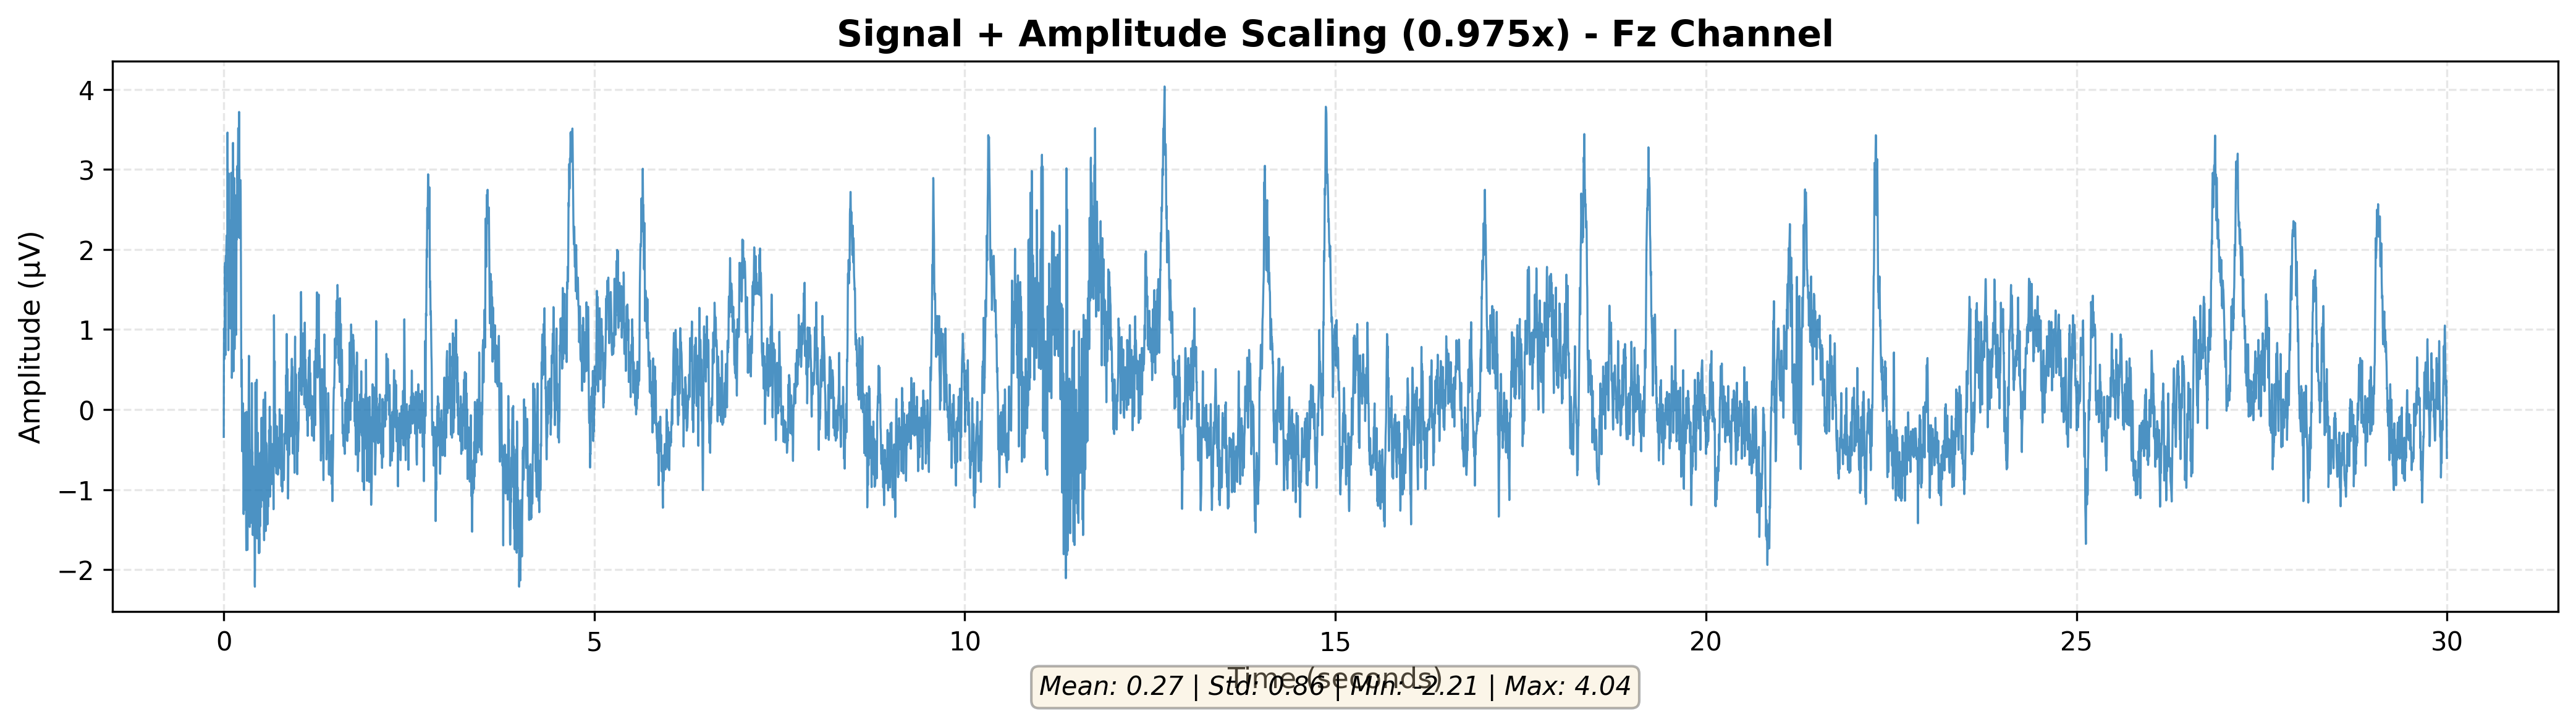
\includegraphics[width=\linewidth]{figure/03_amplitude_scaling.png}
        \caption{Sinyal dengan Amplitude Scaling}
        \label{fig:ampl_sign}
    \end{subfigure}
    
    \caption{Sinyal Augmentasi}
    \label{fig:augmented_signal}
\end{figure}

Sesuai dengan skenario yang telah ditetapkan, proses augmentasi data diterapkan secara dinamis pada setiap iterasi pelatihan untuk memperluas keragaman distribusi data tanpa membebani kapasitas memori. Untuk memverifikasi dampak transformasi terhadap karakteristik fundamental sinyal biologis, dilakukan inspeksi visual dan statistik, seperti yang diilustrasikan pada Gambar \ref{fig:augmented_signal}.

Secara kasat mata, sinyal asli, sinyal dengan penambahan derau (\textit{Gaussian Noise}), dan sinyal yang diskalakan (\textit{Amplitude Scaling}) tampak identik tanpa adanya perubahan bentuk gelombang yang drastis. Hal ini membuktikan bahwa strategi \textit{mild augmentation} yang diterapkan berhasil menjaga integritas fitur temporal dari sinyal EEG. Namun, modifikasi tersebut dapat diamati secara jelas melalui parameter statistik sinyal. 

Pada penambahan \textit{Gaussian Noise} dengan standar deviasi 0.01, terjadi pergeseran minor pada nilai ekstrem amplitudo; nilai minimum bergeser dari -2.27 menjadi -2.28, dan nilai maksimum dari 4.14 menjadi 4.15. Sementara itu, pada penerapan \textit{Amplitude Scaling} dengan faktor pengali 0.975x, rentang amplitudo mengalami penyusutan proporsional, yang ditandai dengan perubahan nilai minimum menjadi -2.21 dan maksimum menjadi 4.04. Meskipun perubahannya sangat kecil secara visual, variasi numerik ini sudah cukup efektif untuk memaksa model Mamba agar tidak menghafal nilai absolut (\textit{overfitting}), melainkan berfokus pada ekstraksi pola dari gelombang kantuk tersebut.

Seluruh proses transformasi probabilitas ini dieksekusi secara terprogram pada tahapan pembacaan data. Detail implementasi algoritma augmentasi tersebut diwujudkan melalui skrip Python yang ditunjukkan pada Kode \ref{code:augmentation} berikut.

\begin{lstlisting}[language=Python, caption=Kode Augmentasi, label={code:augmentation}]
# config.py
USE_AUGMENTATION = True
AUG_GAUSSIAN_NOISE_STD = 0.01
AUG_AMPLITUDE_SCALE_RANGE = (0.9, 1.1)

# datareader.py
class EEGAugmentation:
    def __init__(
        self,
        gaussian_std=Config.AUG_GAUSSIAN_NOISE_STD,
        amplitude_range=Config.AUG_AMPLITUDE_SCALE_RANGE,
        time_shift_max=Config.AUG_TIME_SHIFT_MAX,
        prob=0.5
    ):
        self.gaussian_std    = gaussian_std
        self.amplitude_range = amplitude_range
        self.time_shift_max  = time_shift_max
        self.prob            = prob

    def add_gaussian_noise(self, signal):
        if np.random.rand() < self.prob:
            noise  = torch.randn_like(signal) * self.gaussian_std
            signal = signal + noise
        return signal

    def amplitude_scaling(self, signal):
        if np.random.rand() < self.prob:
            scale  = np.random.uniform(*self.amplitude_range)
            signal = signal * scale
        return signal

# train.py
train_dataset = EEGDataset(
    data_dir=Config.DATA_DIR,
    csv_path=os.path.join('label/labels.csv'),
    fold=fold,
    split='train',
    n_splits=Config.N_SPLITS,
    window_sec=Config.WINDOW_SEC,
    stride_sec=Config.STRIDE_SEC,   
    use_augmentation=Config.USE_AUGMENTATION
)           

val_dataset = EEGDataset(
    data_dir=Config.DATA_DIR,
    csv_path=os.path.join('label/labels.csv'),
    fold=fold,
    split='val',
    n_splits=Config.N_SPLITS,
    window_sec=Config.WINDOW_SEC,
    stride_sec=Config.WINDOW_SEC,   
    use_augmentation=False          
)

train_loader = DataLoader(
    train_dataset
)

val_loader = DataLoader(
    val_dataset
)
\end{lstlisting}

\subsection{Hasil Pelatihan Model}
Setelah seluruh tahapan prapemrosesan dan augmentasi data diselesaikan, model hibrida regresi dan klasifikasi berbasis arsitektur Mamba memasuki tahap pelatihan utama. Proses pelatihan dieksekusi dengan menggunakan \textit{hyperparameter} yang telah dioptimalkan secara empiris guna menjaga keseimbangan antara \textit{convergence rate} dan pencegahan \textit{overfitting}. Rincian \textit{hyperparameter} yang digunakan pada eksperimen ini dirangkum pada Tabel \ref{tab:hyperparameter}.

\begin{table}[H]
    \centering
    \caption{Konfigurasi \textit{Hyperparameter} Pelatihan Model Mamba}
    \label{tab:hyperparameter}
    \begin{tabular}{lc}
        \hline
        \textbf{Parameter} & \textbf{Nilai} \\
        \hline
        \textit{Epoch} Maksimal & 50 \\
        \textit{Batch Size} & 32 \\
        \textit{Optimizer} & AdamW \\
        \textit{Learning Rate} & $1 \times 10^{-4}$ \\
        \textit{Weight Decay} & $1 \times 10^{-2}$ \\
        \textit{Early Stopping Patience} & 10 \textit{epoch} \\
        LR \textit{Scheduler} & ReduceLROnPlateau \\
        \hline
    \end{tabular}
\end{table}

Proses optimasi model menggunakan \textit{optimizer} AdamW dengan \textit{Weight Decay} sebesar $1 \times 10^{-2}$ sebagai bentuk regulariasi untuk mengurangi ketergantungan model pada \textit{noise} sinyal. Strategi pelatihan dilengkapi dengan \textit{Learning Rate Scheduler} menggunakan metode \textit{ReduceLROnPlateau}, yang secara otomatis menurunkan laju pembelajaran saat nilai \textit{loss} validasi mengalami stagnasi guna mencapai konvergensi yang lebih halus. Selain itu, diterapkan mekanisme \textit{Early Stopping} dengan \textit{patience} sebanyak 10 \textit{epoch} untuk menghentikan pelatihan saat tidak terjadi perbaikan performa, sehingga mencegah \textit{overfitting} dan memastikan model tersimpan pada kondisi optimal.

Sebagai representasi visual dari dinamika pembelajaran model, Gambar \ref{fig:4.loss-regression} menampilkan kurva penurunan kerugian (\textit{loss curve}) untuk target regresi yang dievaluasi menggunakan \textit{Mean Absolute Error} (MAE). Grafik ini diambil dari \textit{Fold} ke-1 hingga ke-5.

\begin{figure}[H]
    \centering
    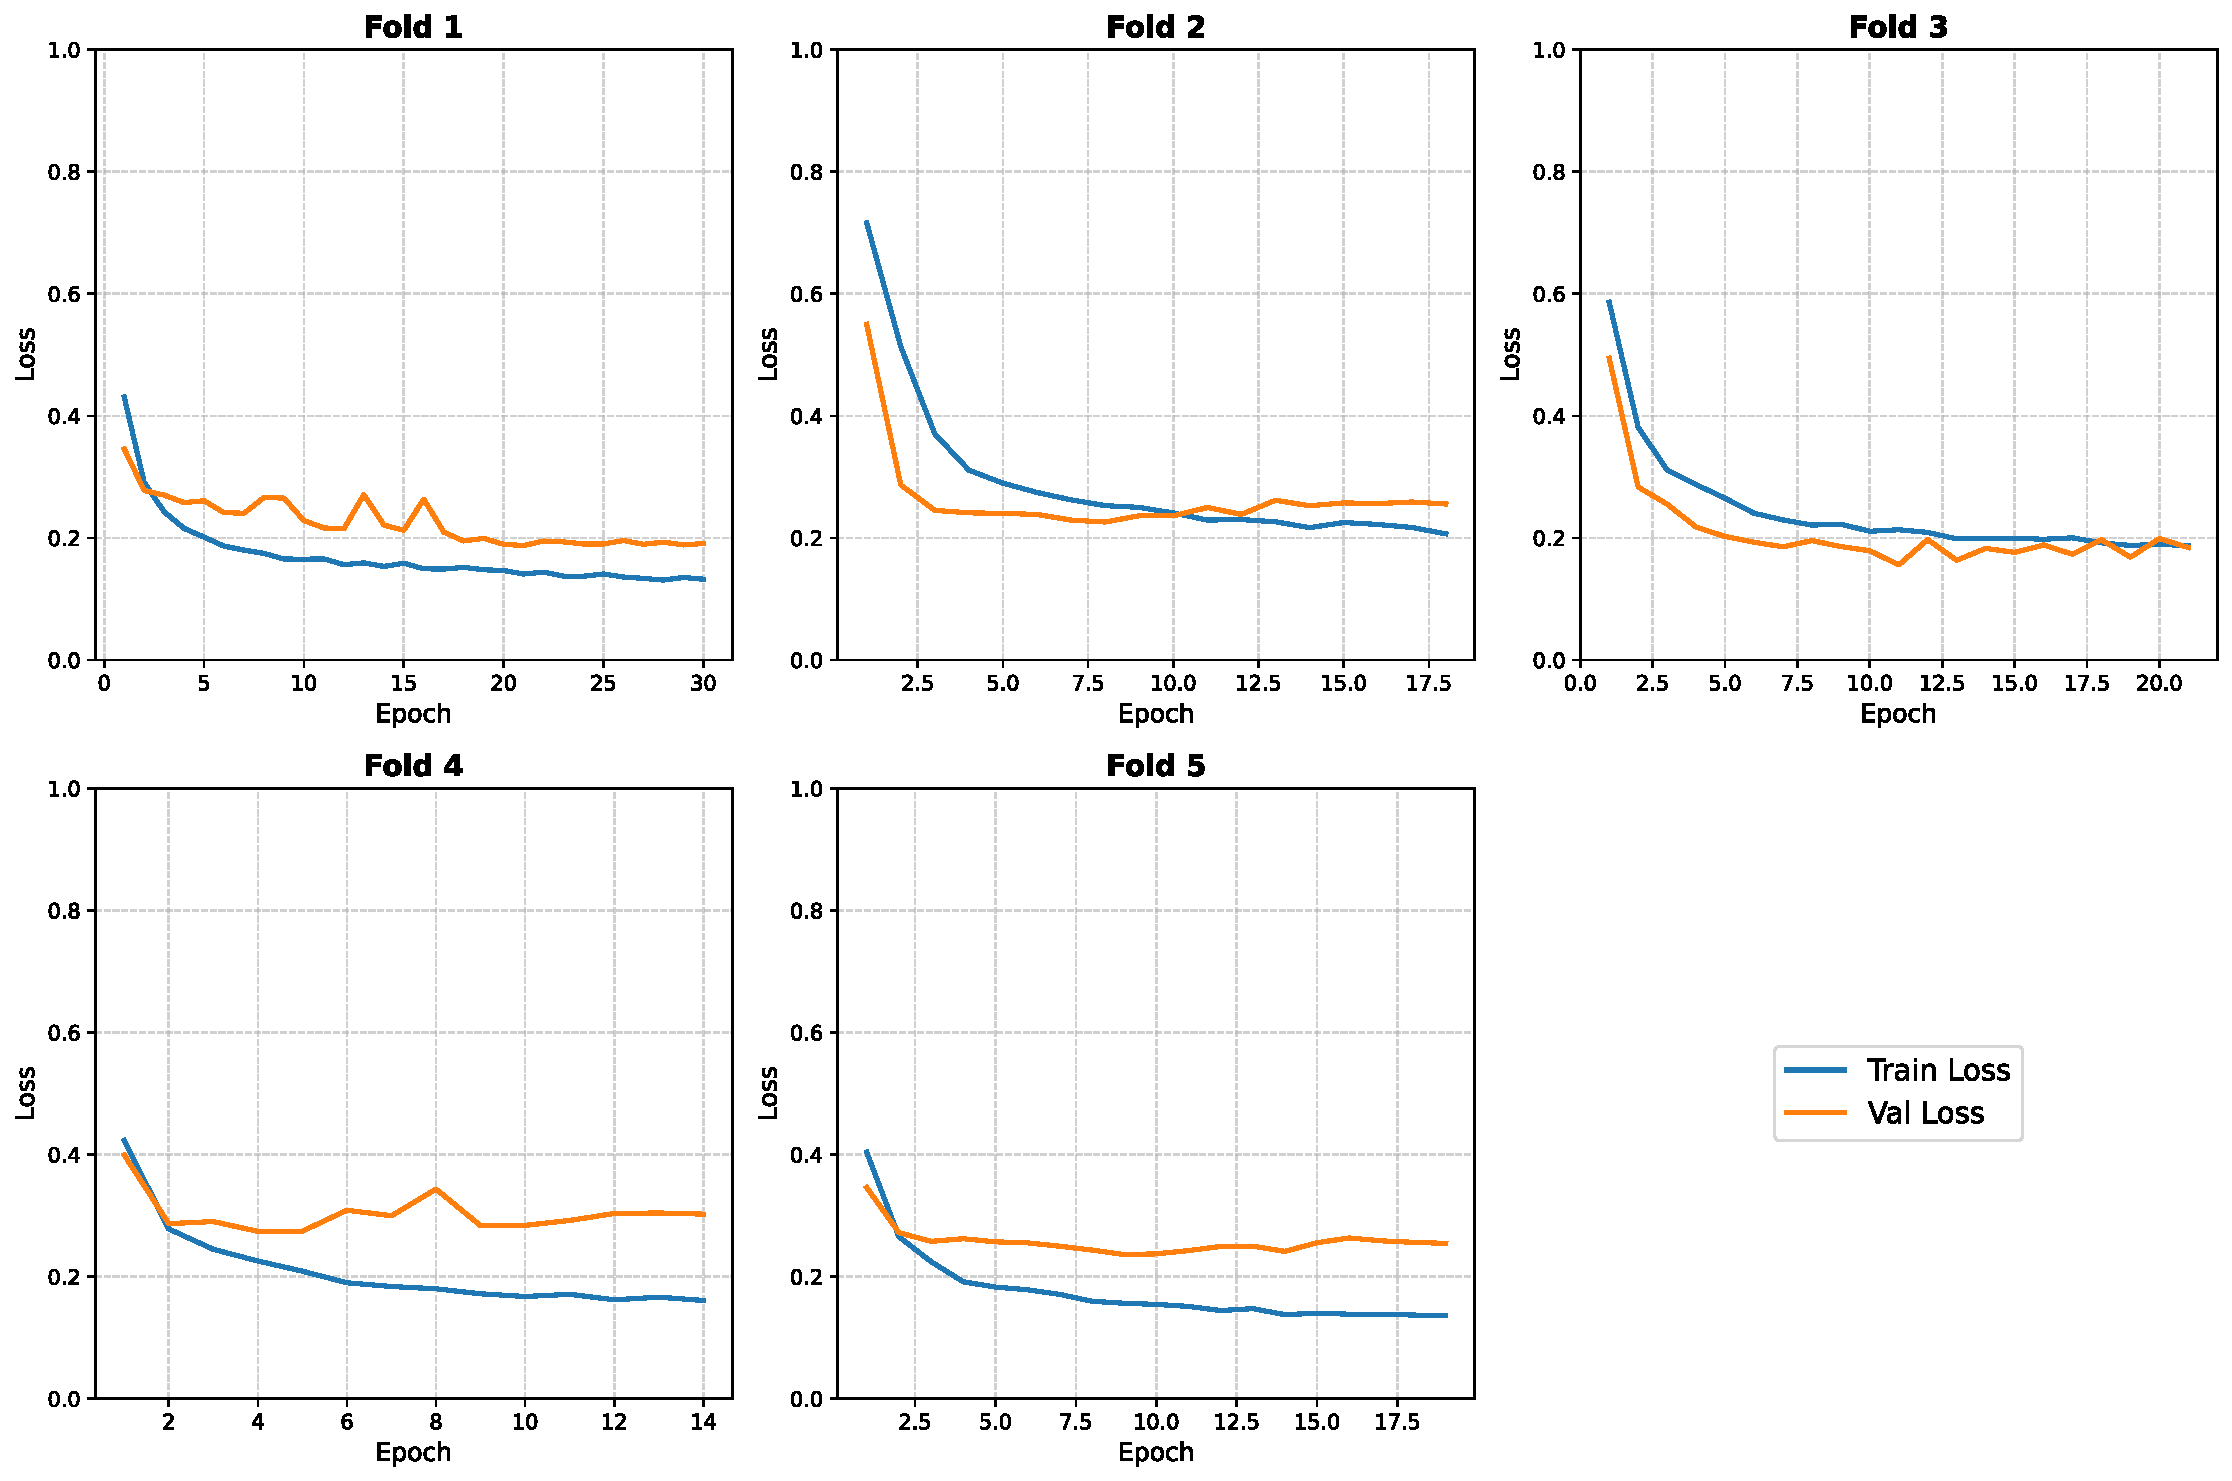
\includegraphics[width=10cm]{figure/loss-regression.pdf}
    \caption{Grafik Loss Pendekatan Regresi}
    \label{fig:4.loss-regression}
\end{figure}

Berdasarkan visualisasi keseluruhan grafik \textit{loss} dari kelima \textit{fold} pengujian tersebut, dapat diamati bahwa nilai \textit{training loss} secara konsisten mengalami penurunan yang signifikan dan mulus hingga mencapai titik stabil di kisaran 0.15 hingga 0.20 pada akhir \textit{epoch}. Sementara itu, kurva \textit{validation loss} secara umum juga mengikuti tren penurunan yang searah dan mampu berkonvergensi dengan baik di kisaran angka 0.20 hingga 0.30. Meskipun terdapat fluktuasi minor pada kurva validasi di beberapa \textit{fold}, hal tersebut merupakan karakteristik wajar akibat tingginya kompleksitas dan variabilitas data sinyal fisiologis antar-individu. Jarak yang relatif sempit dan stabil antara kurva latih dan kurva validasi di seluruh \textit{fold} ini menjadi bukti empiris bahwa cabang regresi pada arsitektur Mamba berhasil mengekstrak fitur temporal secara efektif tanpa mengalami \textit{overfitting}. Hal ini sekaligus mengonfirmasi keberhasilan fungsi regularisasi \textit{Weight Decay} yang diterapkan dalam menjaga stabilitas generalisasi model di berbagai variasi data subjek.

Berbeda dengan target regresi, cabang klasifikasi pada model menunjukkan dinamika pelatihan yang lebih menantang. Gambar \ref{fig:4.loss-classification} menampilkan kurva kerugian untuk target klasifikasi yang dievaluasi menggunakan \textit{Weighted Cross-Entropy Loss}.

\begin{figure}[H]
    \centering
    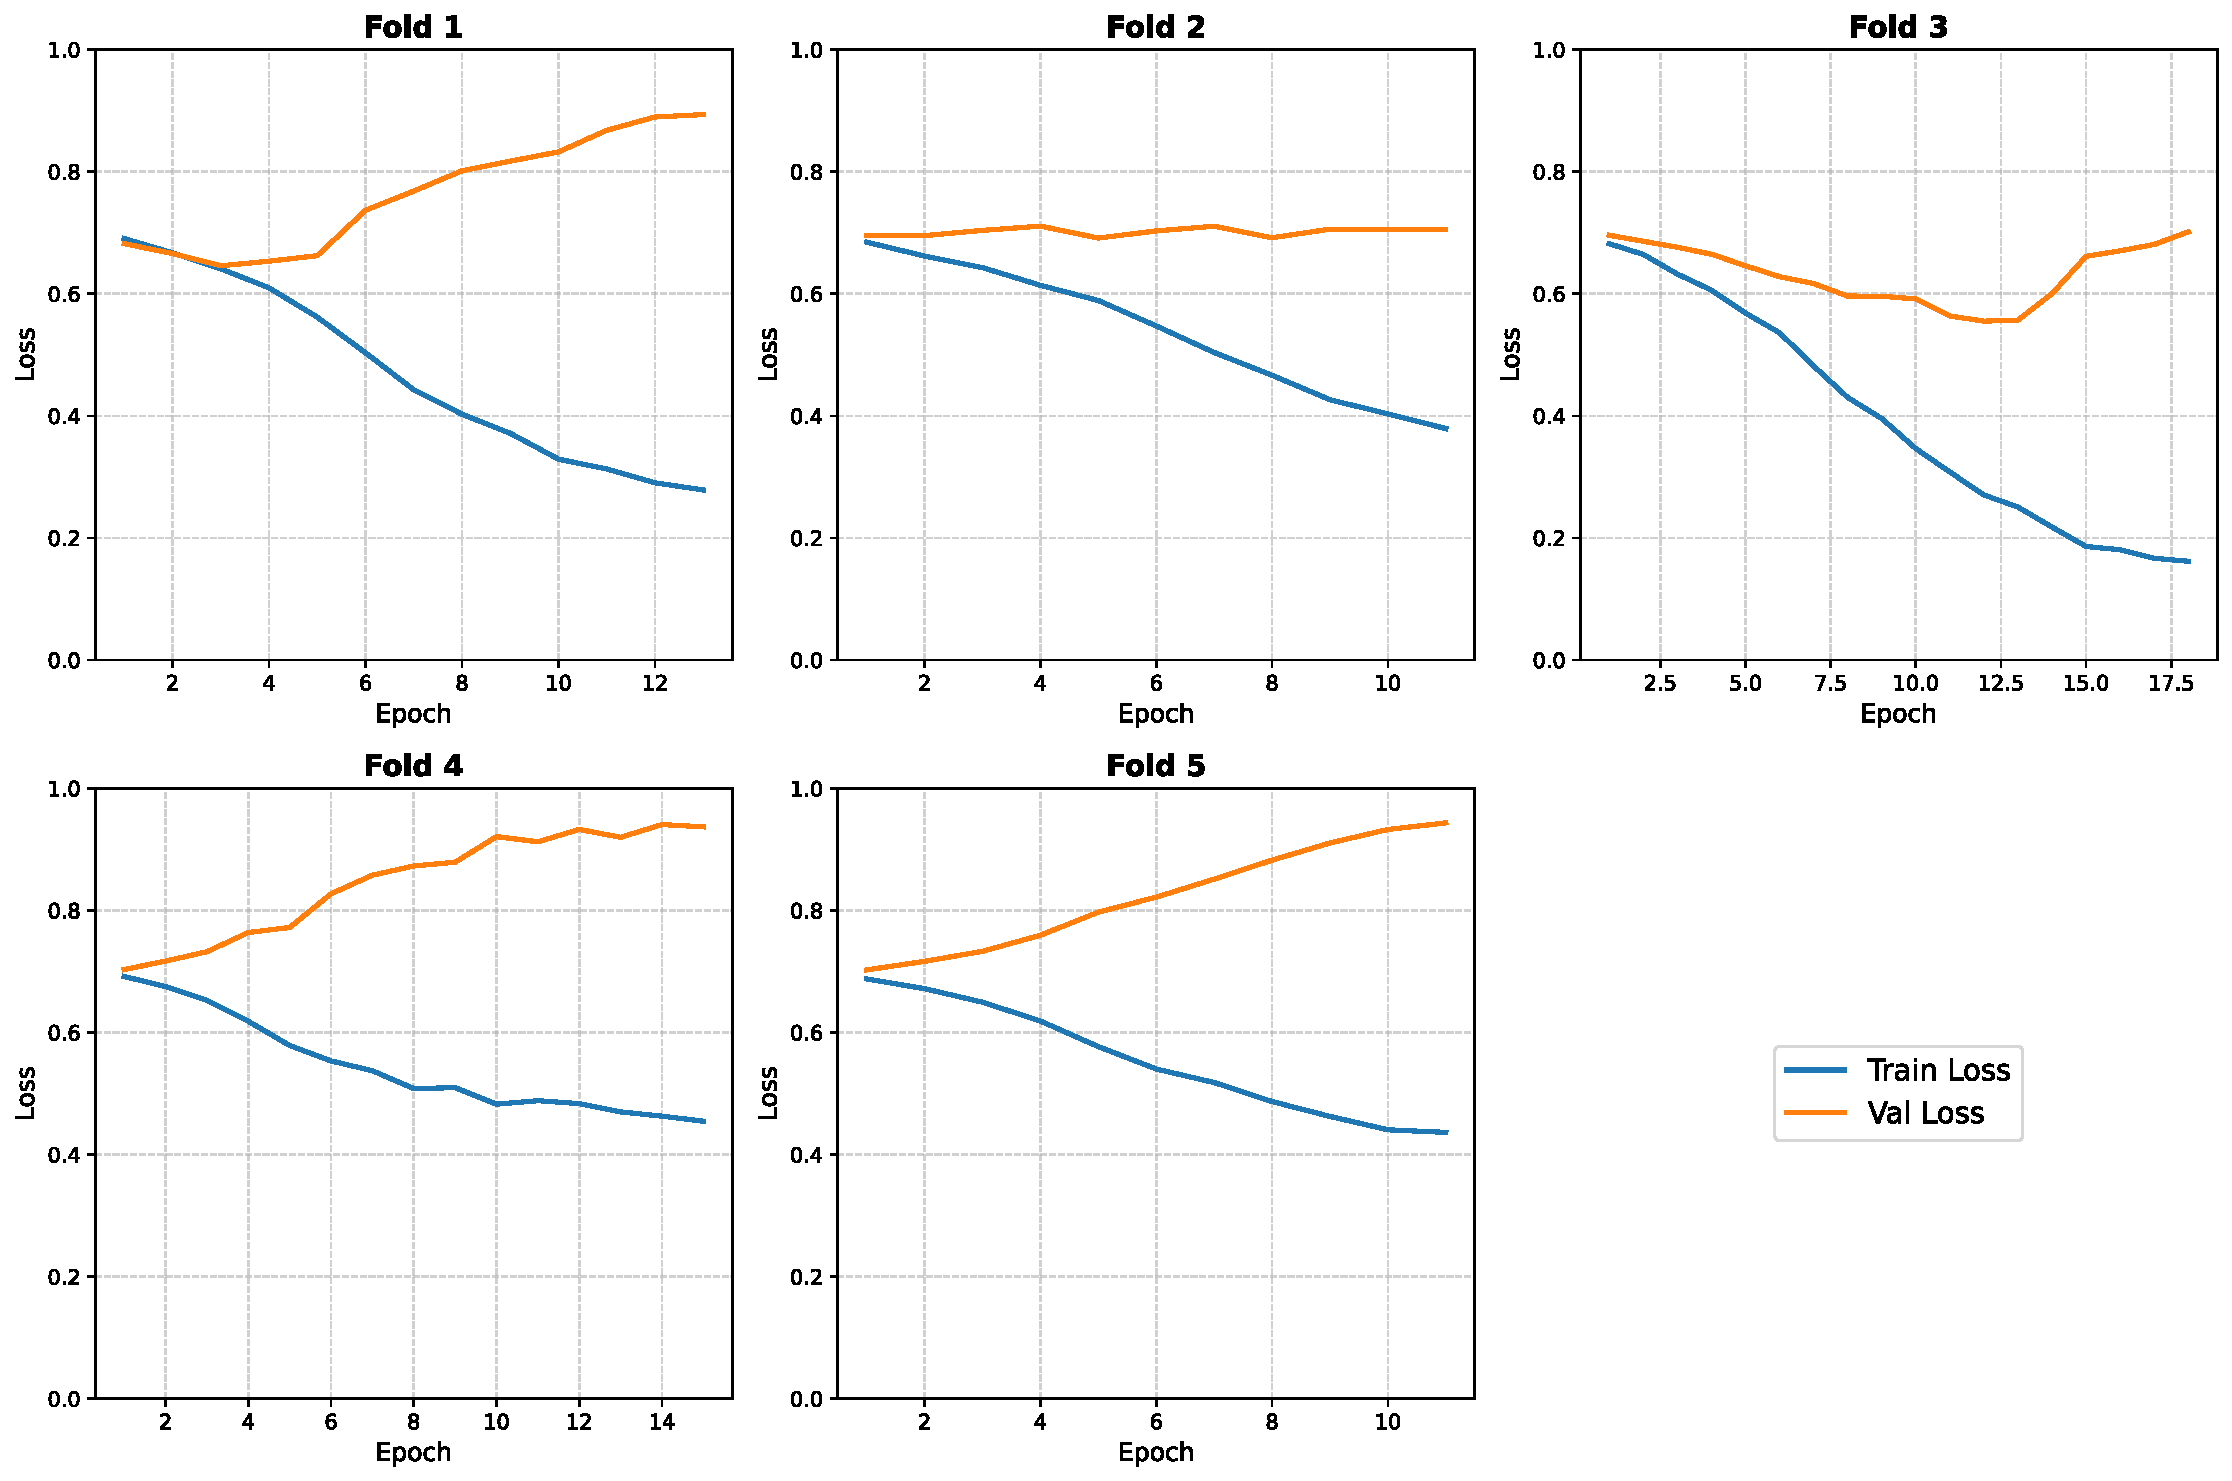
\includegraphics[width=10cm]{figure/loss-classification.pdf}
    \caption{Grafik Loss Pendekatan Klasifikasi}
    \label{fig:4.loss-classification}
\end{figure}

Berdasarkan visualisasi keseluruhan grafik \textit{loss} dari kelima \textit{fold} pengujian tersebut, terlihat pola umum di mana \textit{training loss} selalu berhasil menurun secara konsisten. Namun, kurva \textit{validation loss} mayoritas menunjukkan tren peningkatan pada titik \textit{epoch} yang bervariasi, seperti setelah \textit{epoch} ke-5 pada Fold 1, setelah \textit{epoch} ke-12 pada Fold 3, hingga tren yang langsung meningkat sejak awal pelatihan pada Fold 4 dan 5. Fenomena kenaikan yang terjadi secara sistematis di hampir seluruh \textit{fold} ini sangat dipengaruhi oleh tingginya variabilitas karakteristik sinyal antar-subjek, serta perbedaan karakteristik matematis antara kedua fungsi kerugian yang digunakan. Pada cabang regresi, MAE menghitung selisih kesalahan secara absolut dan \textit{linier}, sehingga penalti yang diberikan terhadap prediksi yang meleset tetap proporsional dan menjaga kurva tetap stabil.

Sebaliknya, pada cabang klasifikasi biner, model dituntut untuk membuat keputusan kategori yang kaku dan tegas. Fenomena lonjakan \textit{validation loss} ini sangat dipengaruhi oleh sifat fungsi kerugian yang memberikan hukuman besar pada batas transisi antar-kelas. Sebagai perbandingan, pada skenario regresi, jika skor KSS aktual subjek adalah 5 namun model memprediksi 6, kesalahan tersebut hanya dihitung sebagai selisih kecil yang proporsional sehingga kurva tetap stabil. Namun pada skenario klasifikasi, jika skor aktual adalah 5 (kategori \textit{Alert}) dan fitur model sedikit bergeser menyerupai skor 6 (kategori \textit{Drowsy}), model akan langsung dianggap melakukan kesalahan fatal karena tebakannya menyeberang ke kelas yang berbeda. Mengingat transisi fisiologis sinyal kantuk pada dataset DROZY terjadi secara bertahap dan sangat halus, model kerap kali terjebak pada batas tipis ini saat memproses data validasi dari subjek baru. Pemberian penalti yang besar akibat "salah kamar" pada batas transisi inilah yang menyebabkan akumulasi \textit{validation loss} melonjak tajam secara visual, meskipun secara fisiologis tebakan model sebenarnya hanya meleset tipis dari ambang batas.

\section{Hasil Evaluasi Kinerja Model} \label{IV.Hasil_Uji}
Evaluasi kinerja model dieksekusi menggunakan skema \textit{5-Fold Cross-Validation} untuk memastikan bahwa performa yang dihasilkan bersifat objektif dan tidak bias terhadap porsi pembagian data tertentu. Mengingat arsitektur Mamba yang diusulkan memiliki dua cabang keluaran (regresi dan klasifikasi), evaluasi dilakukan secara terpisah untuk membandingkan efektivitas kedua pendekatan tersebut dalam mendeteksi tingkat kantuk.

\subsection{Kinerja Pendekatan Regresi}
Pada cabang regresi, model bertugas memprediksi nilai \textit{Karolinska Sleepiness Scale} (KSS) dalam rentang kontinu 1 hingga 9. Untuk dapat membandingkan kinerjanya dengan tugas klasifikasi biner, nilai KSS hasil prediksi regresi dikonversi menggunakan nilai ambang batas (\textit{threshold}) sebesar 5.5, sebagaimana telah dijustifikasi pada bab metodologi. Apabila nilai KSS prediksi $\leq 5.5$, maka sampel dikategorikan sebagai \textit{Alert} (rentang asli 1-5), sedangkan jika nilai $> 5.5$ dikategorikan sebagai \textit{Drowsy} (rentang asli 6-9). Rangkuman hasil evaluasi regresi untuk kelima \textit{fold} disajikan pada Tabel \ref{tab:hasil_regresi}.

\begin{table}[H]
    \centering
    \caption{Hasil Evaluasi 5-Fold Cross-Validation pada Target Regresi}
    \label{tab:hasil_regresi}
    \begin{tabular}{cccc}
        \hline
        \textbf{Fold} & \textbf{MAE (Skala 1-9)} & \textbf{Akurasi Threshold (\%)} & \textbf{F1-Score} \\
        \hline
        1 & 1.6926 & 64.91 & 0.6429 \\
        2 & 1.9560 & 54.39 & 0.3158 \\
        3 & 1.5990 & 63.91 & 0.5385 \\
        4 & 2.3994 & 53.80 & 0.2883 \\
        5 & 2.1225 & 50.53 & 0.5524 \\
        \hline
        \textbf{Rata-rata} & \textbf{1.9539 $\pm$ 0.2902} & \textbf{57.51 $\pm$ 6.48} & \textbf{0.4676 $\pm$ 0.1566} \\
        \hline
    \end{tabular}
\end{table}

Berdasarkan Tabel \ref{tab:hasil_regresi}, model mencapai rata-rata MAE sebesar 1.9539. Perlu dicatat bahwa meskipun model dilatih menggunakan target KSS yang dinormalisasi ke rentang 0-1, perhitungan metrik evaluasi MAE akhir dilakukan setelah mengembalikan nilai prediksi dan target ke skala KSS asli (1-9) melalui proses \textit{inverse transform} (dikalikan dengan nilai maksimum 9.0). Hal ini dilakukan agar nilai \textit{error} dapat diinterpretasikan secara langsung. Angka MAE ini menunjukkan bahwa prediksi model secara umum meleset sekitar 2 poin dari skor KSS aktual subjek. Meskipun terdapat variansi performa antar-\textit{fold}, stabilitas MAE yang berada di bawah angka 2.5 membuktikan bahwa model mampu mengikuti tren perubahan sinyal EEG dan EOG secara bertahap. Namun, ketika hasil regresi dikonversi menjadi klasifikasi biner, rata-rata akurasi yang dihasilkan adalah 57,51\% ($\pm$ 6,48\%) dengan F1-Score sebesar 0,4676 ($\pm$ 0,1566). Tingginya angka standar deviasi ini menjadi indikasi awal adanya fluktuasi performa yang dipengaruhi oleh karakteristik subjek pada masing-masing \textit{fold}. Di samping variansi tersebut, rendahnya nilai rata-rata F1-Score juga mengindikasikan adanya ketidakseimbangan model dalam mendeteksi kelas tertentu, yang diperjelas melalui analisis \textit{Confusion Matrix} pada Gambar \ref{fig:4.cm-regression}.

\begin{figure}[H]
    \centering
    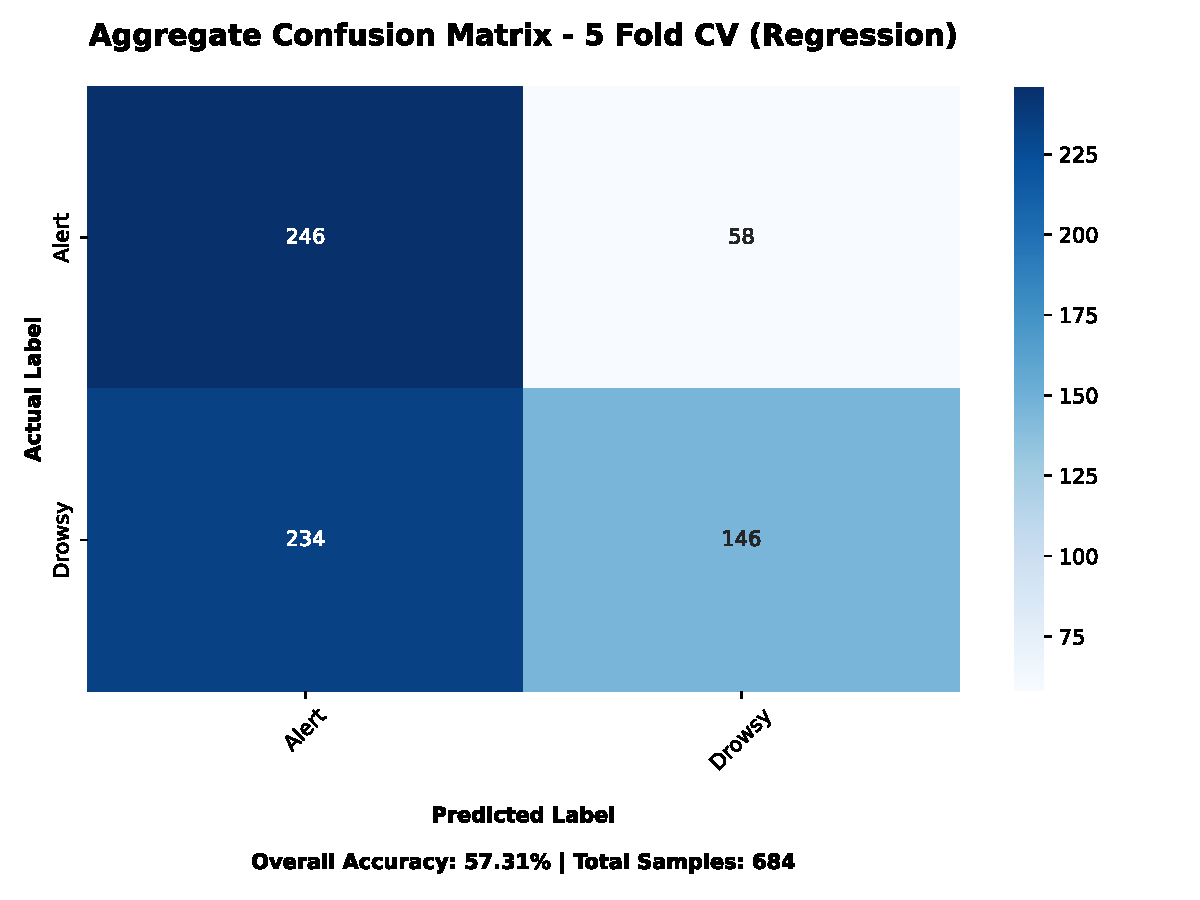
\includegraphics[width=10cm]{figure/cm_aggregate_regression.pdf}
    \caption{Confusion Matrix Agregasi Pendekatan Regresi}
    \label{fig:4.cm-regression}
\end{figure}

Berdasarkan hasil agregasi \textit{Confusion Matrix} dari kelima \textit{fold} pengujian dengan total 684 sampel, pendekatan regresi menghasilkan akurasi sebesar 57,31\%. Dari Gambar \ref{fig:4.cm-regression} di atas terlihat bahwa model memiliki kecenderungan untuk lebih sering memprediksi kelas sadar (\textit{Alert}). Model berhasil mengenali kondisi \textit{Alert} dengan cukup baik, yaitu 246 prediksi benar dari 304 sampel asli. Namun, kelemahan utama model ini terlihat jelas pada kemampuannya mendeteksi kondisi kantuk (\textit{Drowsy}). Dari 380 sampel yang aslinya \textit{Drowsy}, model hanya mampu memprediksi dengan benar sebanyak 146 sampel, sedangkan 234 sampel lainnya salah diklasifikasikan sebagai \textit{Alert}. Tingginya angka kesalahan ini (\textit{False Negative}) menunjukkan bahwa model regresi terlalu berhati-hati dan lebih memilih untuk "mencari aman" dengan memprediksi kondisi \textit{Alert}. Hal ini membuktikan bahwa penggunaan fungsi kerugian MAE pada model regresi kurang peka dalam menangkap tanda-tanda awal dari rasa kantuk. Meskipun sangat akurat dalam mencegah \textit{False Alarm}, pendekatan ini memiliki risiko tinggi karena gagal mendeteksi subjek yang sebenarnya sudah mulai kehilangan kesadaran.

\subsection{Kinerja Pendekatan Klasifikasi}
Berbeda dengan cabang regresi yang memprediksi nilai kontinu secara bertahap, cabang klasifikasi pada arsitektur Mamba dilatih secara khusus menggunakan \textit{Weighted Cross-Entropy Loss} untuk langsung memisahkan sinyal ke dalam dua kelas biner (\textit{Alert} dan \textit{Drowsy}). Hasil evaluasi performa klasifikasi dari kelima \textit{fold} dirangkum secara mendetail pada Tabel \ref{tab:hasil_klasifikasi}.

\begin{table}[H]
    \centering
    \caption{Hasil Evaluasi 5-Fold Cross-Validation pada Target Klasifikasi}
    \label{tab:hasil_klasifikasi}
    \begin{tabular}{ccc}
        \hline
        \textbf{Fold} & \textbf{Akurasi (\%)} & \textbf{F1-Score} \\
        \hline
        1 & 80.70 & 0.7512 \\
        2 & 61.99 & 0.5485 \\
        3 & 69.17 & 0.6860 \\
        4 & 60.23 & 0.5698 \\
        5 & 57.89 & 0.3667 \\
        \hline
        \textbf{Rata-rata} & \textbf{66.00 $\pm$ 8.26} & \textbf{0.5844 $\pm$ 0.1319} \\
        \hline
    \end{tabular}
\end{table}

Berdasarkan Tabel \ref{tab:hasil_klasifikasi}, pendekatan klasifikasi murni menghasilkan rata-rata akurasi sebesar 66,00\% ($\pm$ 8,26\%). Jika dibandingkan dengan rata-rata akurasi hasil \textit{thresholding} regresi (57,51\%), angka ini secara keseluruhan terlihat lebih tinggi. Namun, nilai rata-rata F1-Score yang hanya sebesar 0,5844 ($\pm$ 0,1319) menunjukkan adanya masalah keseimbangan dalam prediksi. Besarnya rentang standar deviasi pada metrik ini mengonfirmasi bahwa performa model sangat fluktuatif. Model mampu memprediksi dengan tingkat keberhasilan yang tinggi di beberapa \textit{fold}, namun performanya merosot tajam di \textit{fold} lainnya akibat perbedaan karakteristik subjek yang diuji. Untuk memahami detail distribusi kesalahan dan bagaimana performa model secara keseluruhan, kita perlu melihat agregasi tebakan model pada \textit{Confusion Matrix} di Gambar \ref{fig:4.cm-classification}.

\begin{figure}[H]
    \centering
    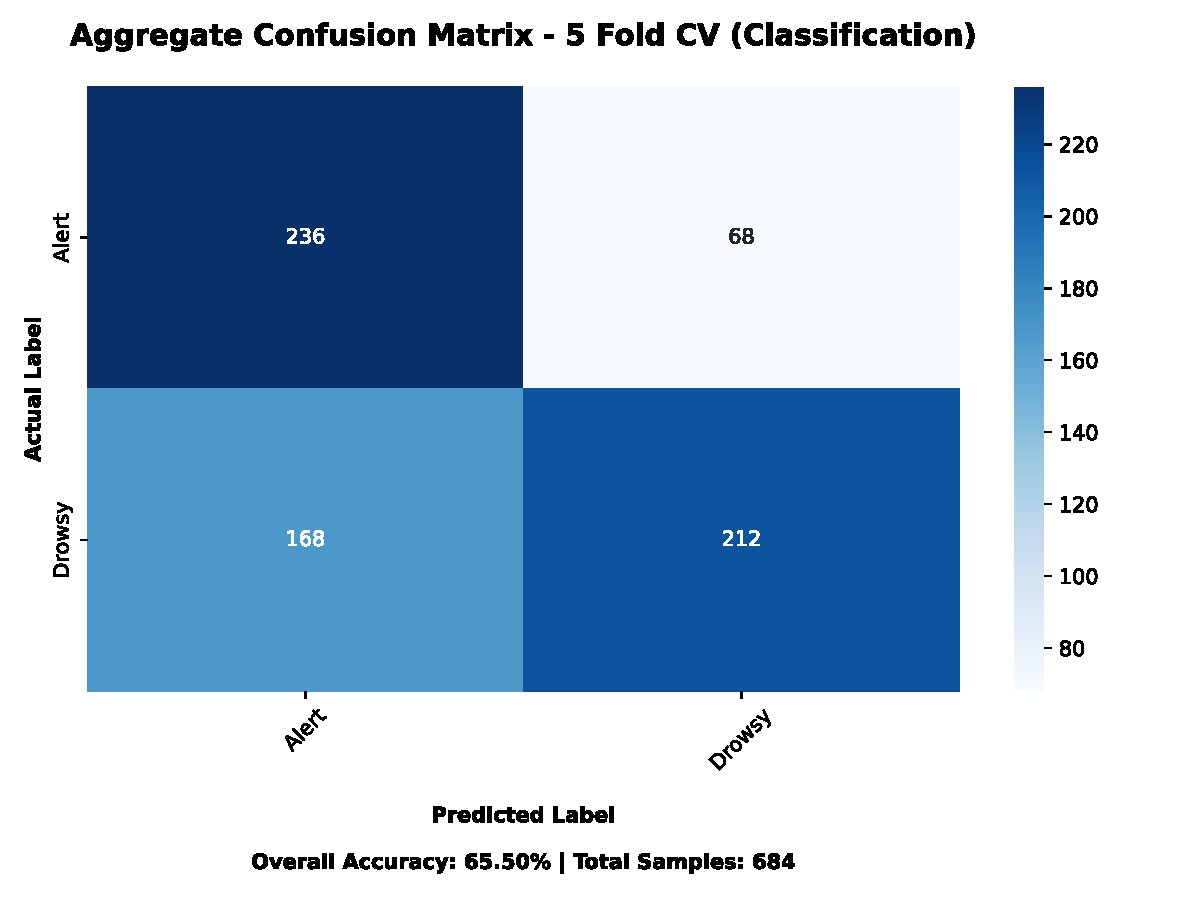
\includegraphics[width=10cm]{figure/cm_aggregate_classification.pdf}
    \caption{Confusion Matrix Agregasi Pendekatan Klasifikasi}
    \label{fig:4.cm-classification}
\end{figure}

Hasil agregasi \textit{Confusion Matrix} pada pendekatan klasifikasi biner menunjukkan kinerja yang lebih seimbang dengan tingkat akurasi yang lebih tinggi, yaitu 65,50\%. Berdasarkan Gambar \ref{fig:4.cm-classification}, penggunaan fungsi kerugian \textit{Weighted Cross-Entropy} terbukti mampu membuat model lebih fokus untuk mengenali kelas \textit{Drowsy}. Jumlah prediksi benar untuk kondisi kantuk meningkat secara nyata menjadi 212 sampel, jauh lebih baik dibandingkan dengan pendekatan regresi. Sebagai risikonya, model ini menjadi sedikit lebih sensitif sehingga memunculkan lebih banyak alarm palsu (\textit{False Positive}), di mana terdapat 68 sampel \textit{Alert} yang salah diprediksi sebagai \textit{Drowsy}. Walaupun masih ada 168 sampel kantuk yang belum berhasil terdeteksi, secara keseluruhan pendekatan klasifikasi ini memberikan distribusi prediksi yang lebih merata. Pendekatan klasifikasi dinilai lebih sesuai untuk sistem peringatan keselamatan karena lebih sigap dan tanggap dalam menangkap indikasi pengemudi yang mulai mengantuk.

Dapat disimpulkan bahwa kedua pendekatan ini memiliki karakter yang bertolak belakang. Model regresi cenderung sangat berhati-hati dan memprioritaskan untuk meminimalkan salah prediksi subjek sadar sebagai mengantuk, meskipun risikonya adalah banyak subjek yang sebenarnya mengantuk justru terlewat. Sementara itu, model klasifikasi bertindak lebih responsif dengan fokus untuk "menangkap sebanyak mungkin" indikasi kantuk, walaupun hal ini memicu sedikit peningkatan pada jumlah alarm palsu. Perbedaan performa yang kontras ini membuktikan bahwa mendeteksi transisi kantuk dari sinyal EEG dan EOG merupakan tugas yang sangat menantang. Batas fisiologis antara kondisi sadar dan mulai mengantuk sangatlah tipis, sehingga secara tidak langsung model dipaksa untuk memilih sebuah kompromi: menjadi terlalu berhati-hati seperti pada pendekatan regresi, atau lebih agresif seperti pada klasifikasi.

\subsection{Perbandingan Metrik Per-Kelas}

Untuk memperoleh pemahaman yang lebih mendalam mengenai karakteristik prediksi masing-masing pendekatan, evaluasi dilakukan pada tingkat per-kelas menggunakan data agregasi dari kelima \textit{fold} pengujian. Tabel~\ref{tab:per_class_metrics} menyajikan nilai \textit{precision}, \textit{recall}, dan \textit{F1-score} untuk setiap kelas pada kedua pendekatan secara terpisah.

\begin{table}[H] % Pakai [H] dari package float biar stay 
\centering
\caption{Perbandingan Metrik Per-Kelas Pendekatan Regresi dan Klasifikasi}
\label{tab:per_class_metrics}
\renewcommand{\arraystretch}{1.2} % Kasih jarak antar baris biar gak sesek
\setlength{\tabcolsep}{10pt} % Lebarin jarak antar kolom
\begin{tabular}{llccc}
\toprule
\textbf{Pendekatan} & \textbf{Kelas} & \textbf{Precision} & \textbf{Recall} & \textbf{F1-Score} \\
\midrule
\multirow{3}{*}{Regresi}
    & \textit{Alert}         & 0,5125 & 0,8092 & 0,6277 \\
    & \textit{Drowsy}        & 0,7157 & 0,3842 & 0,4998 \\ \cmidrule(lr){2-5}
    & \textbf{Macro Avg}     & \textbf{0,6141} & \textbf{0,5967} & \textbf{0,5638} \\
\midrule
\multirow{3}{*}{Klasifikasi}
    & \textit{Alert}         & 0,5842 & 0,7763 & 0,6666 \\
    & \textit{Drowsy}        & 0,7571 & 0,5579 & 0,6425 \\ \cmidrule(lr){2-5}
    & \textbf{Macro Avg}     & \textbf{0,6707} & \textbf{0,6671} & \textbf{0,6546} \\
\bottomrule
\end{tabular}
\end{table}

Berdasarkan Tabel~\ref{tab:per_class_metrics}, terdapat pola yang sangat kontras antara kedua pendekatan dalam mendeteksi masing-masing kelas. Pada pendekatan regresi, model menunjukkan nilai \textit{recall} yang tinggi untuk kelas \textit{Alert} (0{,}8092), namun \textit{recall} kelas \textit{Drowsy} hanya mencapai 0{,}3842. Artinya, dari seluruh sampel yang sebenarnya berstatus mengantuk, model regresi hanya mampu mengidentifikasi dengan benar sekitar 38,42\% di antaranya. Kondisi ini secara langsung mengkonfirmasi temuan pada analisis \textit{confusion matrix} sebelumnya, bahwa model regresi berperilaku layaknya \textit{conservative classifier} yang cenderung memilih prediksi \textit{Alert} sebagai opsi yang lebih aman.

Sebaliknya, pendekatan klasifikasi menunjukkan distribusi metrik yang jauh lebih seimbang antar kelas. Nilai \textit{recall} kelas \textit{Drowsy} meningkat secara signifikan menjadi 0{,}5579 dibandingkan pendekatan regresi, yang berarti model klasifikasi mampu mendeteksi lebih dari separuh kondisi kantuk yang sesungguhnya. Sebagai konsekuensinya, nilai \textit{precision} kelas \textit{Alert} mengalami penurunan dari 0{,}5125 menjadi 0{,}5842 yang mengindikasikan adanya peningkatan jumlah \textit{false alarm} dibandingkan pendekatan regresi.

Dari perspektif \textit{macro average}, pendekatan klasifikasi
mengungguli regresi pada seluruh metrik agregat: \textit{precision} (0{,}6707 vs. 0{,}6141), \textit{recall} (0{,}6671 vs. 0{,}5967), dan \textit{F1-score} (0{,}6546 vs. 0{,}5638). Perlu dicatat bahwa nilai \textit{macro F1-score} agregat ini dihitung dari data gabungan kelima \textit{fold} dan berbeda dari rata-rata F1-score per-\textit{fold} yang dilaporkan pada Tabel~\ref{tab:hasil_regresi} dan~\ref{tab:hasil_klasifikasi}. Perbedaan ini wajar secara metodologis karena jumlah sampel per \textit{fold} tidak seragam, sehingga agregasi langsung dan rata-rata aritmetika per-\textit{fold} akan menghasilkan angka yang sedikit berbeda.

\section{Analisis Efisiensi Komputasi} \label{IV.Analisis}
Keunggulan utama dari penggunaan arsitektur Mamba dalam penelitian ini adalah efisiensi komputasinya yang sangat tinggi. Evaluasi efisiensi dilakukan dengan mengukur parameter struktural model dan beban operasional saat melakukan inferensi. Ringkasan metrik efisiensi model disajikan pada Tabel \ref{tab:efisiensi}.

\begin{table}[H]
    \centering
    \caption{Metrik Efisiensi Komputasi Arsitektur Mamba}
    \label{tab:efisiensi}
    \begin{tabular}{ll}
        \hline
        \textbf{Parameter Efisiensi} & \textbf{Nilai} \\
        \hline
        Total Parameter & 62.930 unit \\
        Ukuran File Model (.pth) & 820 KB \\
        Operasi Komputasi (GFlops) & 0,01 \\
        \hline
    \end{tabular}
\end{table}

Berdasarkan Tabel \ref{tab:efisiensi}, model Mamba yang dikembangkan memiliki total parameter sebesar 62.930 unit. Jumlah parameter ini dikategorikan sebagai arsitektur yang sangat ringan (\textit{lightweight}), mengingat model klasifikasi standar umumnya memiliki jutaan parameter. Sehingga model sangat kompetitif untuk dijalankan pada perangkat dengan sumber daya terbatas \textit{(Edge Device)}.

Dari sisi beban operasional, model ini mencatatkan nilai komputasi sebesar 0,01 GFlops. Nilai yang sangat rendah ini menunjukkan bahwa model dapat memproses sinyal EEG/EOG dengan sangat cepat tanpa membebani unit pemroses grafis (GPU). Dengan demikian, arsitektur Mamba terbukti memenuhi syarat efisiensi untuk aplikasi pemantauan kondisi pengemudi secara berkelanjutan dengan konsumsi daya yang minimal.

\section{Perbandingan dengan \textit{Baseline}}
Untuk mengevaluasi performa model secara menyeluruh, hasil pengujian Mamba pada penelitian ini dibandingkan dengan model pembanding \textit{baseline} dari Cao et al. (2025) \cite{Cao2025Optimized}. Model tersebut dipilih sebagai pembanding utama karena sama-sama menggunakan dataset DROZY \cite{Massoz2016} untuk kasus deteksi kantuk. Walaupun menggunakan dataset yang sama, perlu dicatat bahwa perbandingan ini tidak sepenuhnya \textit{apple-to-apple}. %
Hal ini dikarenakan model pembanding menggunakan pendekatan \textit{multimodal}, sedangkan penelitian ini murni menggunakan pendekatan \textit{single-modal} dengan arsitektur Mamba. Selain perbedaan modalitas, informasi mengenai jumlah parameter dan beban komputasi tidak disebutkan secara eksplisit di dalam jurnal pembanding tersebut. Oleh karena itu, estimasi nilai komputasi pada model \textit{baseline} didapatkan dengan cara mereplikasi ulang arsitekturnya berdasarkan deskripsi struktural yang dilaporkan penulisnya. Meskipun hasil replikasi ini mungkin tidak seratus persen identik dengan kode aslinya, kerangka makro yang dibangun sudah sangat mendekati dan dinilai cukup valid untuk digunakan sebagai acuan komparasi. Pada akhirnya, perbandingan ini tetap penting dilakukan untuk melihat seberapa jauh model Mamba bisa lebih efisien secara komputasi dan seberapa layak model ini diterapkan untuk sistem deteksi kantuk secara \textit{real-time} yang membutuhkan proses ringan. %

\begin{table}[H]
    \centering
    \caption{Perbandingan Kinerja dan Efisiensi Komputasi Model}
    \label{tab:perbandingan_model}
    \renewcommand{\arraystretch}{1.2} % Kasih napas antar baris
    \small % Perkecil sedikit biar teks panjang muat dengan elegan
    \begin{tabular}{lccc}
        \hline
        \textbf{Metrik Evaluasi} & \textbf{\begin{tabular}[c]{@{}c@{}}Model Pembanding\\ (Cao et al.)\end{tabular}} & \textbf{\begin{tabular}[c]{@{}c@{}}Model Usulan\\ (Klasifikasi)\end{tabular}} & \textbf{\begin{tabular}[c]{@{}c@{}}Model Usulan\\ (Regresi)\end{tabular}} \\
        \hline
        Modalitas Input    & Multimodal & \textit{Single-modal} & \textit{Single-modal} \\
        Arsitektur Utama   & ResNet18 + LSTM & Mamba (4 Layer) & Mamba (4 Layer) \\
        Akurasi           & 98,41\% & 66,00\% & 57,51\% \\
        F1-Score          & 0,9838 & 0,5844 & 0,4676 \\
        Total Parameter   & 11,57 juta & 62.930 unit & 62.930 unit \\
        Beban Komputasi   & 0,27 GFlops & 0,01 GFlops & 0,01 GFlops \\
        \hline
    \end{tabular}
\end{table}

Berdasarkan tabel \ref{tab:perbandingan_model}, terlihat adanya \textit{trade-off} yang signifikan antara akurasi dan efisiensi komputasi. Model \textit{multimodal} pembanding terbukti mampu menghasilkan akurasi klasifikasi yang sangat tinggi (98,41\%), namun pencapaian tersebut menuntut beban komputasi yang berat, yakni sekitar 0,27 GFLOPs dengan ukuran model mencapai 11,57 juta parameter. Hal ini disebabkan oleh penggunaan lapisan konvolusi dalam (ResNet18) untuk memproses matriks gambar 2D. Sebaliknya, model Mamba yang diusulkan dalam penelitian ini menawarkan efisiensi komputasi yang ekstrem. Dengan julah parameter yang sangat kecil (62.930 unit) dan beban komputasi yang jauh lebih ringan (0,01 GFLOPs), model ini memberikan alternatif pendekatan \textit{lightweight} dalam memproses sinyal EEG/EOG. Efisiensi ini menjadikan model Mamba memiliki potensi sumber daya terbatas (\textit{edge devices}) di dalam kendaraan, yang mana kecepatan inferensi dan konsumsi daya yang rendah menjadi prioritas utama.

Selain perbedaan pada modalitas, perbedaan hasil metrik ini juga dipengaruhi oleh konteks \textit{setup} eksperimen. Model pembanding melakukan ekstraksi fitur gambar wajah secara bersamaan dengan pemrosesan sinyal fisiologis, yang secara inheren memberikan lebih banyak petunjuk visual seperti kondisi mata yang terpejam atau posisi kepala secara langsung kepada model. Di sisi lain, model pada penelitian ini lebih fokus untuk melihat kemampuan asli arsitektur Mamba dalam memproses data sinyal fisiologis secara berurutan. Penggunaan teknik pemotongan data dan CNN (\textit{Temporal CNN Feature Extractor}) di awal proses terbukti sangat membantu meringankan beban kerja model. Langkah ini berhasil memangkas proses komputasi tanpa membuang informasi penting dari pola gelombang otak (EEG) dan gerakan mata (EOG). Pada akhirnya, walaupun tingkat akurasi yang didapat untuk skema klasifikasi dan regresi belum melampaui model \textit{multimodal}, studi ini berhassil membuktikan bahwa Mamba bisa berjalan dengan sumebr daya komputasi yang jauh lebih hemat dan efisien. 

\section{Analisis Hasil Penelitian}

\subsection{Analisis Karakteristik Regresi dan Klasifikasi}
\label{subsec:analisis_karakteristik}

Berdasarkan perbandingan hasil evaluasi, terlihat bahwa kedua pendekatan dalam arsitektur Mamba ini menampilkan karakteristik yang sangat bertolak belakang akibat perbedaan fungsi kerugian yang digunakan. Cabang regresi yang dilatih dengan fungsi kerugian MAE terbukti memiliki kecenderungan lebih berhati-hati. Tingginya tingkat deteksi pada kondisi \textit{Alert} bukanlah indikator keunggulan mutlak, melainkan dampak dari kehati-hatian model dalam memberikan prediksi skor tinggi, sehingga model berperilaku layaknya \textit{majority class classifier}. Sifat ini membuat model regresi sangat minim menghasilkan \textit{False Alarm}, namun kurang optimal untuk dijadikan sistem peringatan dini karena rentan melewatkan fase awal kantuk.

Di sisi lain, cabang klasifikasi yang dilatih menggunakan \textit{Weighted Cross-Entropy} menunjukkan sifat yang lebih tanggap dan agresif dalam mendeteksi kondisi \textit{Drowsy}. Fungsi pembobotan kelas berhasil memaksa model untuk lebih memprioritaskan kelas minoritas atau kondisi bahaya, meskipun hal ini membawa risiko peningkatan kesalahan prediksi (\textit{False Alarm}) pada subjek yang sebenarnya masih sadar.

Selain dari metrik evaluasi akhir (Akurasi dan F1-Score), kontradiksi karakteristik kedua pendekatan ini juga sangat jelas terlihat pada dinamika kurva kerugian (\textit{loss curve}) selama proses pelatihan. Secara angka performa biner, pendekatan klasifikasi memang lebih unggul, namun grafik \textit{validation loss}-nya (Gambar \ref{fig:4.loss-classification}) justru menunjukkan tren fluktuatif dan akumulasi \textit{error} yang meningkat. Sebagaimana dijelaskan sebelumnya, lonjakan ini bukanlah indikasi bahwa model gagal belajar, melainkan konsekuensi dari sifat pembagian kelas yang kaku. Model kerap menerima penalti kesalahan yang maksimal ketika prediksi fitur sinyalnya hanya meleset tipis melewati ambang batas kategori. Tingginya lonjakan \textit{loss} ini mengonfirmasi betapa sulitnya memisahkan batas kondisi sadar dan mengantuk secara tegas pada data EEG dan EOG akibat transisi yang sangat halus.

Sebaliknya, meskipun menghasilkan metrik klasifikasi biner yang lebih rendah setelah melalui proses konversi, pendekatan regresi menampilkan dinamika pembelajaran yang jauh lebih sehat dan stabil secara grafik yang dapat dilihat pada Gambar \ref{fig:4.loss-regression}. Karena fungsi kerugian MAE hanya menghitung selisih jarak secara murni, prediksi yang meleset tipis akan tetap dievaluasi sebagai kesalahan kecil yang proporsional, sehingga model terhindar dari lonjakan kurva yang ekstrem. Kontradiksi grafis dan numerik ini memberikan \textit{insight} yang krusial: pendekatan klasifikasi lebih responsif dalam mendeteksi indikasi kantuk namun rentan menerima penalti kerugian besar akibat pergeseran fitur minor di sekitar ambang batas. Sementara itu, pendekatan regresi menawarkan stabilitas pelatihan yang sangat baik, namun harus mengorbankan sensitivitas deteksi bahaya karena sifat tebakannya yang cenderung mencari aman.

\subsection{Analisis Efektivitas Mekanisme \textit{Selective State Space}}
\label{subsec:analisis_mamba_efektivitas}

Keberhasilan model dalam mencapai rata-rata akurasi yang kompetitif dengan jumlah parameter yang sangat minimal, yaitu hanya sebesar 62.930 unit, merupakan bukti kuat efektivitas mekanisme \textit{Selective State Space} yang menjadi inti dari arsitektur Mamba. Berbeda dengan model RNN tradisional yang sering mengalami degradasi performa pada urutan data yang panjang, Mamba mampu menjaga aliran informasi temporal penting dari sinyal EEG/EOG sepanjang 15.360 sampel secara efisien.

Kemampuan Mamba dalam melakukan kompresi informasi secara linear menjadi kunci utama mengapa model yang dikembangkan tetap mampu menghasilkan performa yang stabil di tengah tingginya variabilitas antar-subjek (\textit{inter-subject variability}) pada \textit{dataset} DROZY. Hal ini menunjukkan bahwa arsitektur Mamba tidak hanya unggul secara teoritis, tetapi juga sangat aplikatif dalam menangani data sinyal biologis yang kompleks dan \textit{time-series}.

\subsection{Analisis Variansi dan Pengaruh Karakteristik Subjek}
\label{subsec:analisis_variansi}

Berdasarkan Tabel \ref{tab:hasil_regresi} dan Tabel \ref{tab:hasil_klasifikasi}, hasil evaluasi menggunakan 5-\textit{Fold Cross-Validation} menunjukkan adanya variansi performa yang cukup tinggi antar-\textit{fold}. Pada pendekatan klasifikasi, nilai F1-Score berfluktuasi dari angka tertinggi 0,7512 (Fold 1) hingga angka terendah 0,3667 (Fold 5), dengan standar deviasi keseluruhan mencapai $\pm 0,1319$. Tingginya angka variansi ini membuktikan bahwa kemampuan prediksi model masih sangat dipengaruhi oleh subjek yang sedang dievaluasi. 

Investigasi lebih lanjut terhadap penurunan performa yang drastis pada Fold 4 dan Fold 5 mengindikasikan adanya pengaruh kuat dari \textit{inter-subject variability}. Sinyal fisiologis seperti EEG sangat unik untuk setiap individu. Subjek-subjek yang berada pada himpunan uji di Fold 5 kemungkinan besar memiliki pola transisi gelombang otak yang berbeda dari distribusi mayoritas subjek pada data latih.

Dari perspektif implementasi di dunia nyata, tingginya variansi ini memberikan dampak langsung terhadap keandalan sistem. Model yang ada saat ini belum sepenuhnya tangguh (\textit{robust}) untuk digeneralisasikan kepada pengguna baru tanpa adanya penyesuaian. Hal ini mengimplikasikan bahwa sistem deteksi kantuk yang optimal tidak hanya membutuhkan arsitektur yang ringan seperti Mamba, tetapi ke depannya juga memerlukan fase kalibrasi singkat untuk mempelajari sinyal dasar dari masing-masing subjek baru, atau membutuhkan pelatihan dengan dataset berskala jauh lebih besar untuk mencakup seluruh kemungkinan variasi sinyal otak manusia.